% Paper 1 -- Fidetype. arXiv version, 2026-11-12: main text, references, Appendix A and the
% supplementary material (Sections S1-S22) in ONE document, so that all cross-references resolve
% without xr-hyper. Works with pdflatex (arXiv) and Tectonic. Do not edit sections/, generated/ or
% figures/ here: make-arxiv.sh copies them from ../../latex/ and ../../figures/.
% The bibliography is in main.bbl (generated from ../../latex/refs.bib by make-arxiv.sh).
\documentclass[11pt,a4paper]{article}
\usepackage[a4paper,margin=2.5cm]{geometry}
\usepackage[T1]{fontenc}
\usepackage[utf8]{inputenc}
\usepackage{lmodern}
\usepackage{microtype}
\usepackage{amsmath,amssymb}
\usepackage{graphicx}
\usepackage{booktabs}
\usepackage{adjustbox}
\usepackage{enumitem}
\usepackage{multirow}
\usepackage{array}
\usepackage{xcolor}
\usepackage{tikz}
\usetikzlibrary{arrows.meta,positioning,shapes.geometric,fit,calc,backgrounds}
\usepackage[font=small,labelfont=bf]{caption}
\usepackage{subcaption}
\usepackage{placeins}
\usepackage{float}
\usepackage{algorithm}
\usepackage{algpseudocode}
\usepackage[numbers,sort&compress]{natbib}
\usepackage[colorlinks=true,linkcolor=blue!50!black,citecolor=blue!50!black,urlcolor=blue!50!black]{hyperref}
\usepackage{url}
\usepackage{etoolbox}
\usepackage[capitalise,noabbrev]{cleveref}

\graphicspath{{figures/}}
\newcommand{\figdir}{figures/}  % folder of the TikZ figure sources
\emergencystretch=2em

\newcommand{\nts}{NeuralTextStream}
\newcommand{\ewpm}{eWPM}
\newcommand{\act}[1]{\textsc{#1}}
\newcommand{\code}[1]{\texttt{#1}}
\newcommand{\ci}[2]{\ensuremath{[#1,\,#2]}}
\newcommand{\papertitle}{When should a neural text-entry decoder commit?\\Risk-controlled commits from a stream-level trust layer}
% generated table rows: primitive input, so that \midrule may follow inside a tabular
\makeatletter\newcommand{\inputrows}[1]{\@@input #1 }\makeatother

\title{\papertitle}
\author{Zibo Zhang\\[2pt] \normalsize Independent researcher}
\date{}

\begin{document}
\maketitle

\begin{abstract}
\noindent\textit{Objective.} Neural text-entry decoders often end in a language model that writes fluent sentences from weak neural evidence. We ask when such a system should send (\emph{commit}) a sentence without confirmation, and whether wrong commits can be bounded.
\textit{Approach.} A trust layer reads the decoder's per-frame output stream, calibrates its confidence, and commits, offers alternatives or abstains. A Learn-then-Test threshold, never below a speed-tuned threshold, bounds the wrong-commit rate with high probability. The rule was chosen after the random re-splits below; all inference is exploratory. We test it offline on one intracortical speech participant (Brain-to-Text '25, 14 days; our decoder, and the published sentence gated by agreement with it), calibrating before testing in time. Forearm sEMG and MEG typing serve as format and safety checks.
\textit{Main results.} Always committing sent wrong text for 61\% and 19\% of sentences. Calibrated on earlier days, the rule's pooled wrong-commit rate was 1.0--2.7\% (target 5\%); no day was significantly above 5\%. Over 50 random re-splits, 8\% (95\% CI 2--19\%) and 2\% (0.1--11\%) exceeded 5\%; the rule committed 15\% and 39\% of sentences, and 21\% and 8\% of commits were wrong. The bound covers the mix of days: one day ran at 10\%. On our decoder, a plain threshold committed 198 of 300 no-information streams; with an evidence guard, none.
\textit{Significance.} A stream-level commit rule kept wrong commits rare across days for one participant. It needs an input-validity check and per-session calibration, and commits few sentences with current decoders.
\textit{Clinical trial registration:} BrainGate2, ClinicalTrials.gov NCT00912041.
\end{abstract}

\noindent\textbf{Keywords:} brain--computer interface, text entry, language model, risk control, Learn then Test, selective prediction, safety
\medskip
\section{Introduction}
\label{sec:intro}

Brain--computer interfaces (BCIs) for text entry are moving towards clinical and consumer use. Intracortical neuroprostheses decode attempted speech, handwriting and typing at high rates \citep{willett2023speech,card2024accurate,metzger2023avatar,willett2021handwriting,jude2026bimanual}; non-invasive decoders reconstruct typed sentences from magnetoencephalography (MEG) \citep{levy2026brain2qwerty,zhang2026brain2qwertyv2}; and surface electromyography (sEMG) is a candidate input for wearables \citep{sivakumar2024emg2qwerty,achituve2025emg,ctrllabs2025generic}. Most of these systems end in a language-model (LM) stage that turns noisy per-frame predictions into sentences. This lowers the error rate but changes the kind of error: when the neural evidence is weak, the LM still returns a grammatical sentence, and a reader has no cue that it is wrong. In speech recognition, such fluent unsupported output has caused documented harm \citep{koenecke2024careless}.

For people who depend on the interface to communicate, accuracy is a stated priority \citep{huggins2011als,huggins2015sci,blabe2015assessment,kubler2014ucd}, and users of augmentative and alternative communication (AAC) want LM-generated text to reflect their own intent \citep{valencia2023aac,kane2017avuncular}. A sentence sent in their name that they did not mean is a harm in itself. Current speech neuroprostheses read a finalised sentence aloud without a confirmation step \citep{card2024accurate} or synthesise voice instantaneously \citep{wairagkar2025voice}. Whether a decoded sentence should be sent without confirmation (\emph{committed}) is therefore a real design decision.

Sentence-level LM decoders for speech, handwriting, typing and sEMG share one structure: per-frame probabilities followed by an LM search. A commit rule can therefore act on the per-frame output instead of inside one decoder. The statistical tools exist: calibration, selective classification, conformal risk control (CRC) and Learn-then-Test (LTT) \citep{guo2017calibration,geifman2017selective,bates2021rcps,angelopoulos2024crc,angelopoulos2025ltt}. They have been applied to single BCI decoders \citep{kim2025confidence,huang2025cocontrol} and to speech recognition \citep{damri2026risk}. The methods are not new. What is missing is their use as a commit rule for neural text entry, a test of the guarantee when calibration comes before use in time, and the fair comparators: ``always offer, never commit'' and a no-BCI baseline such as gaze typing \citep{cai2024gaze}.

\paragraph{This work.} We define the problem (\cref{sec:setting}), a trust layer on a per-frame output stream (\cref{sec:trust}) and an evaluation protocol (\cref{sec:protocol}), and test them offline on public data. Our contributions are:
\begin{enumerate}[leftmargin=*,itemsep=1pt]
  \item \textbf{A stream-level commit rule with a stated guarantee.} The layer calibrates the per-frame log-probabilities and chooses \act{commit}, \act{offer} or \act{abstain}. LTT with a max rule bounds the wrong-commit rate with high probability (Algorithm~\ref{alg:decide}; Algorithm~\ref{alg:calibrate} in the supplement).
  \item \textbf{A time-ordered test of the guarantee on one participant.} We calibrate on earlier days or on the start of a session and test on later data, over 14 days. We also show the scope of the guarantee: it bounds the risk over the mix of days, not on each day.
  \item \textbf{A safety-first evaluation protocol}: the wrong-commit rate with the commit rate and the error among commits; always-commit, always-offer and gaze-typing baselines; a simulated-user speed metric with a sensitivity analysis; and signal-destroying controls. These controls show that a plain confidence threshold commits no-information streams, so a commit rule needs an input-validity check.
\end{enumerate}
The stream format (\nts{} v0.1), its adapters, an audit log and all scripts are released under Apache-2.0. The sEMG and MEG data show that one format and one code path work across devices; they do not show that the commit rule works across decoders.

\Cref{fig:teaser} summarises the result. On the one intracortical participant, the layer turned frequent wrong commits into rare ones. On composed sEMG sentences it committed few sentences, and on MEG it never committed. Its speed gains over the same policy without commits were small (about 1\% and 3\%) and depend on the user model, and on the published decoder always committing was faster, so our claim is about safety.

\begin{figure}[t]
  \centering
  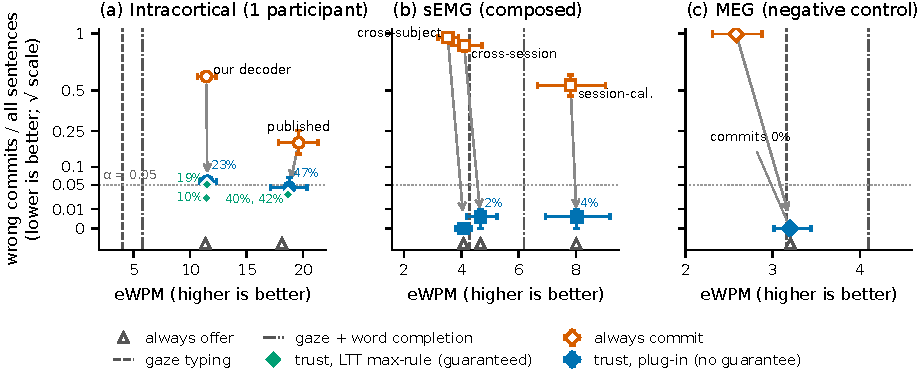
\includegraphics[width=\linewidth]{fig1_teaser.pdf}
  \caption{\textbf{The trust layer turns frequent wrong commits into rare ones; on MEG it does so by never committing.} Wrong commits per sentence attempted (signed square-root axis) against effective words per minute (\ewpm{}) of a simulated user. Open markers: always commit; blue: plug-in trust layer (full fit, no guarantee); green diamonds: the guaranteed rule (fit-A pipeline, guard, clean calibration, LTT max rule; fixed splits A and B); triangles: always offer (no wrong commits; drawn just below 0). Labels give the commit rate. Dashed line: gaze typing; dash-dotted: gaze typing with word completion; dotted: $\alpha = 0.05$. Error bars: 95\% cluster-bootstrap CIs over days (a), participants (b) and sentences $\times$ participants (c), conditional on the fitted pipeline. (a)~Intracortical speech, one participant, 816 test trials. (b)~sEMG, 551 composed sentences, 19 participants; the guaranteed rule gives the same rates as the plug-in rule (not drawn). (c)~MEG typing, 637 instances of 17 sentences; the layer equals always offer.}
  \label{fig:teaser}
\end{figure}

\section{Related work}
\label{sec:related}

\paragraph{Brain-to-text decoders.} MEG decoding of typed sentences reached a CER of 0.29 with a keystroke-locked model \citep{levy2026brain2qwerty}; a second version decodes without key times and adds an LLM stage \citep{zhang2026brain2qwertyv2}. Intracortical decoders reach high accuracy for handwriting, speech and typing \citep{willett2021handwriting,willett2023speech,card2024accurate,metzger2022spelling,jude2026bimanual}, with public phoneme logits \citep{willett2024lessons,card2025data}; sEMG text entry exists for the wrist and forearm \citep{sivakumar2024emg2qwerty,ctrllabs2025generic,achituve2025emg}. Most use CTC \citep{graves2006ctc} with beam search and an LM \citep{hannun2014deepspeech}. In the intracortical study whose data we use, a sentence was finalised after 6\,s without speech or by an eye-gaze button, then read aloud, and the participant rated it afterwards \citep{card2024accurate}. There was no confirmation before text-to-speech, which corresponds to our \act{commit}. Other speech neuroprostheses make the same decision implicitly \citep{moses2021neuroprosthesis,metzger2023avatar,wairagkar2025voice}.

\paragraph{Error handling in BCIs and speech interfaces.} P300 and RSVP spellers commit a character when its posterior passes a threshold \citep{schreuder2013dynamic,throckmorton2013bayesian,mainsah2015dynamic}, often with an LM prior \citep{orhan2012rsvp,oken2014rsvp,speier2016nlp}. Error-related potentials allow automatic error detection \citep{schalk2000errp,ferrez2008errp,spuler2012errp,chavarriaga2014errare}; asynchronous BCIs detect a ``no-control'' state \citep{mason2000asynchronous,zhang2008asynchronous,aloise2011asynchronous}; myoelectric control rejects uncertain decisions \citep{scheme2013rejection}; adaptive decoders change the decoder over days \citep{orsborn2014clda,jarosiewicz2015selfcal,degenhart2020stabilization,fan2023plugandplay,wilson2023recal}. Kim et al.\ accept or abstain on single EEG speech classifications with calibrated ensembles \citep{kim2025confidence}, and Huang et al.\ give calibrated alternatives \citep{huang2025cocontrol}; neither bounds the rate of wrong sentences sent. Speech recognition has a long line of word and utterance confidence measures \citep{jiang2005confidence}, and spoken dialogue systems accept, confirm or reject an utterance by cost-based thresholds \citep{bohus2005error}. Our commit / offer / abstain decision is this accept / confirm / reject decision with a finite-sample bound.

\paragraph{Calibration, selection and risk control.} Temperature scaling fixes over-confidence \citep{guo2017calibration} but degrades under shift \citep{ovadia2019trust}. Selective classification trades coverage for risk; selection with guaranteed risk (SGR) bounds the error among accepted items \citep{geifman2017selective}. CRC bounds the expected value of a monotone loss \citep{angelopoulos2021gentle,angelopoulos2024crc}, LTT bounds a risk with high probability \citep{angelopoulos2025ltt}, weighted variants give approximate bounds under shift \citep{tibshirani2019covariate,barber2023beyond,farinhas2024nonexch}, and online methods give long-run guarantees for any sequence \citep{gibbs2021aci,gibbs2022online,angelopoulos2023pid,feldman2023rolling}. Conformal selection controls the false discovery rate among selected items \citep{jin2023selection}, and conformal alignment applies it to decide when to trust foundation-model outputs \citep{gui2024alignment}; this expected error among selected items is the natural comparator for our error among commits. Conformal methods were applied to speech recognition \citep{ernez2023conformal,damri2026risk} and to LM outputs and abstention \citep{quach2024conformal,mohri2024factuality,abbasiyadkori2024abstention}. We use these methods as published; our contribution is their use and evaluation as a commit rule.

\paragraph{Metrics.} BCI utility metrics \citep{dalseno2010utility} and text-entry metrics \citep{soukoreff2003metrics} charge for corrections, unlike the information transfer rate \citep{wolpaw2002bci}; our \ewpm{} is close to the utility metric. LM prediction speeds up gaze typing \citep{ward2000dasher,cai2024gaze}, but scanning prediction lists has a cost \citep{koester1994wordprediction}.

\section{Problem setting and stream interface}
\label{sec:setting}
\label{sec:format}

\paragraph{Items, streams and actions.} An \emph{item} is one attempt to enter one sentence: a \emph{trial} of the intracortical data, an \emph{instance} (one participant typing one sentence) of the MEG data, or a composed \emph{sentence} of the sEMG data. For item $i$, the decoder emits a stream of $F_i$ frames of log-probabilities $\log p_t(v)$ over $V$ tokens. In our open format, \nts{} v0.1, a stream holds this $F \times V$ array, the frame times, the typed vocabulary and the CTC blank index. A producer must emit the decoder's own, unmodified distribution, and ground-truth text must not appear in the stream. One small adapter per device maps decoder output into the stream; every later step is the same code for all devices, with parameters re-fitted per device (format, conformance suite, adapters and audit log: \cref{app:format}).

An LM search returns $K = 10$ ranked candidate sentences with scores, from which we compute $\hat p_{\mathrm{top1}}$, the calibrated probability of the top candidate. The system then takes one action: \act{commit} the top candidate (sent without further input); \act{offer} up to $k$ candidates for the user to pick; or \act{abstain}, after which the user types with a fallback keyboard. Let $c_i \in \{0,1\}$ indicate that the top candidate differs from the intended sentence (exact match after normalising case and punctuation).

\paragraph{The two error quantities.} Over the $n_{\mathrm{test}}$ test items,
\begin{align}
  \text{wrong-commit rate} &= \#\{\text{wrong commits}\} / n_{\mathrm{test}} \approx \Pr(\text{commit} \wedge \text{wrong}), \\
  \text{error among commits (EAC)} &= \#\{\text{wrong commits}\} / \#\{\text{commits}\} \approx \Pr(\text{wrong} \mid \text{commit}).
\end{align}
The first is the \emph{marginal} risk: how often wrong sentences reach the recipient per sentence attempted. It is monotone in the commit threshold, so CRC and LTT can bound it (\cref{sec:crc}). Committing rarely makes it small, so we always report it with the \emph{commit rate}. The second is the \emph{selective} risk that a user sees in committed text (\cref{sec:selective}). $\alpha = 0.05$ is the target wrong-commit rate, $\beta$ the target error among commits and $\delta = 0.1$ the failure probability of the high-probability guarantees (notation: \cref{tab:notation}).

\section{The trust layer}
\label{sec:trust}

The trust layer reads one stream per item and returns one action. It never reads raw signals or decoder weights. Algorithm~\ref{alg:decide} (Appendix~\ref{app:algorithm}) gives the decision for one item, and Algorithm~\ref{alg:calibrate} the fitting and calibration. All parameters are fitted per device on that device's fit data (fitted values: \cref{tab:settings}; policy grid: \cref{app:settings}).

\subsection{Calibration, candidates, guard and policy}
\label{sec:policy}
Decoder log-probabilities are often over-confident. A frame temperature $\tau_f$ rescales every frame, $\tilde p_t(v) \propto p_t(v)^{1/\tau_f}$; it minimises the cross-entropy of the aligned true tokens at the greedy CTC peaks. It is applied \emph{before} the LM search, so it changes the decoded text as well as the confidence. A sentence temperature $\tau_s$ on the scores of the $K$-best list gives $\hat p_{\mathrm{top1}} = \mathrm{softmax}(\text{scores}/\tau_s)_1$; it minimises the binary negative log-likelihood of ``the top candidate is right'' \citep{guo2017calibration}.

Candidates come from a CTC prefix beam search with a character 6-gram LM trained on Tatoeba sentences \citep{graves2006ctc,hannun2014deepspeech}; for intracortical speech, a phoneme beam search is followed by a CMUdict lexicon, a word unigram and the same character LM. Each character of the top candidate gets an acoustic confidence from the calibrated frame posteriors. A \emph{guard} scores how much of the top candidate the LM invented: the larger of the share of characters with acoustic confidence below 0.5 (\emph{low evidence}) and one minus the posterior-weighted word agreement between the top candidate and the top five. The policy takes, in this order: \act{abstain} if the guard risk is at least $r_{\mathrm{abst}}$; \act{commit} if $\hat p_{\mathrm{top1}} \ge \lambda$ and the guard risk is at most $r_{\mathrm{max}}$; \act{offer} a split-conformal sentence set if it has between 1 and $k_{\max}$ candidates; otherwise a fallback. Its thresholds maximise \ewpm{} (\cref{sec:protocol}) on fit data, subject to a fit-data wrong-commit rate of at most $\alpha$. This \emph{plug-in} fit has no guarantee on new data. A \emph{plain threshold} is the same policy without the guard.

The guard was part of the configuration fixed before the evaluation. On real intracortical data it did not lower the wrong-commit rate. On no-information streams it was the only part that stopped commits in the reported fits (\cref{sec:res-null}), so we keep it as an input-validity check. It acts only when the fitted $r_{\max}$ is below 1.0 (\cref{app:guardlimit}).

\paragraph{Gate on a published sentence: a two-decoder agreement signal.} For the published intracortical decoder we have the stream and the published LM-rescored sentence, but not the decoder's scores, LM or weights. We put the published sentence on top of the $K$-best list of our own phoneme-to-word decoder, which runs on the same stream, with a score equal to our best score plus a bonus of 2.0, and give each published word the acoustic confidence of the aligned word in our top candidate. The confidence of a published sentence is therefore a measure of agreement between the two decoders; it is not a stream-only confidence of the published decoder. The published sentence alone gives the layer no signal, and it then never commits (\cref{app:bonus}). The bonus of 2.0 was set by hand when the gate was first written (commit \code{3fb8154}) and was never tuned; bonuses from 0.5 to 4 change the main rows little (\cref{tab:bonus}).

\subsection{Finite-sample control of the wrong-commit rate}
\label{sec:crc}
The commit score $s_i$ is $\hat p_{\mathrm{top1}}$ if the other policy rules allow a commit, and $-\infty$ otherwise. The layer commits when $s_i \ge \lambda$, with loss $L_i(\lambda) = c_i\,\mathbf{1}[s_i \ge \lambda]$. $L_i$ is non-increasing in $\lambda$, and ``never commit'' ($\lambda = +\infty$) has loss 0. On $n$ calibration items with known truth and empirical risk $\hat R_n(\lambda)$:
\begin{itemize}[leftmargin=*,itemsep=1pt]
  \item \textbf{CRC} \citep{angelopoulos2024crc} chooses the smallest $\lambda$ among the calibration scores and $+\infty$ with $\tfrac{n}{n+1}\hat R_n(\lambda) + \tfrac{1}{n+1} \le \alpha$. If the calibration items and a new item are exchangeable, $\mathbb{E}[L_{n+1}(\hat\lambda_{\mathrm{CRC}})] \le \alpha$ over the calibration draw and the new item. This bounds a mean; a single calibration set can exceed $\alpha$. CRC never commits for $n < 19$. Because $\hat\lambda_{\mathrm{CRC}}$ is a minimum over a finite set of scores, the bound holds for the rule ``commit if $s \ge \hat\lambda$'' as implemented, and test items below the lowest eligible calibration score are never committed.
  \item \textbf{LTT} \citep{angelopoulos2025ltt} tests $H_0(\lambda)\colon R(\lambda) > \alpha$ along one fixed, pre-specified sequence from $\lambda = 1.00$ down to $0.00$ in steps of 0.01, with the exact binomial p-value $\Pr(\mathrm{Bin}(n,\alpha) \le n\hat R_n(\lambda))$, and stops at the first non-rejection; $\hat\lambda_{\mathrm{LTT}}$ is the last rejected $\lambda$. Fixed-sequence testing needs no multiplicity correction. If the calibration items are i.i.d.\ from a distribution $P$, then $\Pr\bigl(R_P(\hat\lambda_{\mathrm{LTT}}) \le \alpha\bigr) \ge 1 - \delta$. LTT cannot commit below $n = 45$.
  \item \textbf{Max rule.} The deployed threshold is $\max(\lambda_{\mathrm{tuned}}, \hat\lambda)$, where $\lambda_{\mathrm{tuned}}$ is the plug-in threshold. A larger threshold has a pointwise smaller loss, so both guarantees carry over. ``Pure'' CRC or LTT drop $\lambda_{\mathrm{tuned}}$.
\end{itemize}

\paragraph{Scope of the guarantee.} $P$ is the distribution that the calibration items come from. In our data it is a mixture of days (intracortical) or participants (sEMG). LTT therefore bounds the risk averaged over that mixture. It does not bound the risk on each day, and a user meets one session at a time (\cref{sec:res-perday}). Per-session control needs per-session (Mondrian) calibration, with at least 45 calibration items per session for LTT, or a calibration block at the start of each session.

\paragraph{Primary rule.} Our primary rule is LTT with the max rule, calibrated on clean data. The theory gives an a-priori reason (a high-probability bound instead of a mean), but we chose it in the third revision of our analysis plan, after we saw the random re-splits of \cref{sec:res-resplits}; it is exploratory like every other result here. CRC with the max rule is reported next to it.

\subsection{Controllers for the error among commits}
\label{sec:selective}
The rules above do not bound the error among commits. Its selective risk $\Pr(\text{wrong} \mid s \ge \lambda)$ is not monotone in $\lambda$, so a max rule does not keep a selective bound. Our reference selective controller is \emph{LTT-sel}: on the fixed grid $\lambda = 0.05, 0.10, \ldots, 1.00$ it tests $H_0(\lambda)\colon \Pr(\text{wrong} \mid s \ge \lambda) > \beta$ with the exact binomial p-value given the $n_\lambda$ calibration commits, with a Bonferroni correction over the 20 points, and takes the smallest rejected $\lambda$. \emph{Joint LTT} tests both targets at once: $H_0(\lambda)\colon R(\lambda) > \alpha$ or $\Pr(\text{wrong} \mid s \ge \lambda) > \beta$, with $p(\lambda) = \max(p_{\mathrm{marg}}, p_{\mathrm{sel}})$, the same grid and Bonferroni. With probability at least $1 - \delta$, both risks at the chosen $\lambda$ are within target. For comparison we report SGR \citep{geifman2017selective}, whose guarantee is the one stated in their Theorem~3.2; its bisection chooses the tested thresholds from the data. A selective bound conditions on committing, so it needs many calibration commits.

\paragraph{Separate data.} Both guarantees need the parts that define $s_i$ to be fitted on data disjoint from the calibration items. The protocol ensures this, with four exceptions (\cref{app:separate}): on Brain-to-Text '25 the word-decoder grid was tuned on fit trials that later fall into calibration or test sets (fixed splits and random re-splits); the MEG checkpoint was selected on validation data that include the calibration sentences; and sEMG session-calibrated uses two cross-fitted decoders. An online controller that re-tunes the threshold from user feedback is a safeguard with a long-run guarantee (\cref{app:online}).

\section{Evaluation protocol}
\label{sec:protocol}

\subsection{Outcomes, user model and baselines}
The primary safety outcome is the wrong-commit rate, always reported with the commit rate and the error among commits. Speed is secondary. We simulate a user who reads the output, accepts or corrects a commit, picks from an offer, or types the sentence with a fallback keyboard. For item $i$ with intended sentence $y_i$, the simulation returns the total time $t_i$ and the final text, and
\begin{equation}
  \text{\ewpm{}} = 60 \cdot \frac{\sum_i \mathbf{1}[\text{final text}_i = y_i]\;\mathrm{words}(y_i)}{\sum_i t_i}.
\end{equation}
Like the BCI utility metric \citep{dalseno2010utility}, \ewpm{} charges the time needed to fix errors. A \emph{silent error} is a wrong final text that the user did not correct; we report its rate separately.

The main user types with a gaze keyboard at 20 characters per minute and scans and selects one of $k = 3$ word alternatives in 4.5\,s. The typing speed was measured in one eye-gaze user with ALS, and the 4.5\,s are close to the 4.7\,s measured in the same study \citep{cai2024gaze}; all other costs are assumptions (\cref{tab:user}). After a \act{commit}, the user misses each wrong word with probability 0.05; after an \act{offer}, the main user sees every error. This asymmetry favours offers and is not measured. The neural input runs at 159.3 (intracortical), 75.8 (sEMG) and 152 (MEG) characters per minute. The intracortical rate is the number of characters of the cue sentences divided by the sum of the \code{speech\_duration\_s} field of the data file. The file does not say whether this field includes the 6\,s finalisation pause of the original interface, and we add no time for that pause, which favours the neural input. Because only two costs are measured, we refit every policy under eight user-model variants (\cref{app:user}).

\emph{Baselines:} always commit the top candidate; always offer and never commit; the \emph{same fitted policy without commits} (the same fit-A pipeline and policy with $\lambda = +\infty$, so every item takes the policy's non-commit path), which is the paired comparator for the speed of a commit rule; the plain threshold; gaze typing alone (error-free, which favours it); and gaze typing with \emph{word completion}, where the keyboard shows the three most frequent words with the typed prefix (a context-free unigram).

\subsection{Datasets}
\paragraph{Intracortical speech (Brain-to-Text '25).} The public copy-task file holds the online phoneme CTC logits, cue sentences and published LM-rescored sentences of participant T15 of the BrainGate2 clinical trial \citep{card2024accurate,card2025data}. We use the 1,628 trials with the 125,000-word vocabulary (14 post-implant days, 30--208 trials each). The file has no time stamps, so the file order within each day is the trial order. We evaluate our phoneme-to-word decoder (test WER 0.149) and the published sentence (WER 0.043), gated as in \cref{sec:policy}. A trial is ``wrong'' if the top sentence differs from the cue; the file has no per-trial participant ratings, so we cannot check this label against the participant's own judgement.

\paragraph{Forearm sEMG and MEG typing.} The Toronto sEMG data hold isolated key presses from 19 participants over two days \citep{achituve2025emg,achituve2024data}. We compose held-out Tatoeba sentences from single presses with oracle timing and no inter-key context (570 fit, 551 test sentences), under three decoder conditions: \emph{session-calibrated}, \emph{cross-session} and \emph{cross-subject}. In the SpanishBCBL MEG data, healthy participants typed memorised Spanish sentences \citep{levy2026brain2qwerty,spanishbcbl}; our asynchronous decoder gets no key times at inference, and the test set has 637 instances of 17 sentences (\cref{app:meg}). We use sEMG and MEG to test the stream format and the safety of the layer on weak decoders, not to test the commit rule across decoders.

\subsection{Calibration data and deployment tests}
\label{sec:splits}
The \emph{deployment protocol} calibrates on data that played no other role: a fit-A part fits the temperatures, conformal sets, guard and policy, and a disjoint calibration part only calibrates.

\paragraph{Fixed splits.} On Brain-to-Text '25 the pipeline is fitted on the first half of each day (812 trials) and tested on the second half (816). Each day's fit trials are split into fit-A (411 trials) and clean calibration (401), by alternating trials (split A) or by taking the earlier half as fit-A (split B). On sEMG, 142 fit sentences fit the policy and 143 calibrate; on MEG, 6 validation sentences fit and 5 calibrate.

\paragraph{Time-ordered (forward-chaining) tests.} A real deployment calibrates on earlier data and runs on later data. On Brain-to-Text '25 we therefore fit, calibrate and test in day order: (V1) fit on days $1..k{-}2$, calibrate on day $k{-}1$, test on day $k$; (V4) fit on days $1..k{-}3$, calibrate on days $k{-}2$ and $k{-}1$; (V2) fit once on days 1--3, calibrate on all earlier non-fit days; (V3, session start) fit on days $1..k{-}1$, calibrate on the first half of day $k$ and test on its second half. These give 10--13 test days per design. sEMG has no session order (sentences are composed from presses drawn at random), so it has no time-ordered test.

\paragraph{Random re-splits.} We also repeat the protocol 50 times with random assignments. On Brain-to-Text '25, each re-split permutes every day's trials and splits them day-stratified into fit-A (1/4), clean calibration (1/4) and test (1/2); on sEMG, each participant's fit sentences are re-split into fit-A, policy and calibration parts, with the fixed 551 test sentences, so the sEMG spread is fit and calibration variation only. To cache decodes, the fitted frame temperature was rounded to a step of 0.02 (Brain-to-Text '25) or 0.01 (sEMG); the largest relative change was 0.27\% (Brain-to-Text '25) and 0.38\% (sEMG). Calibration and test items are exchangeable by construction, so these re-splits are a Monte-Carlo check of the theorems on one pool of data, not a deployment test. Their spread is split-to-split variation, not a CI for new data. We also report the \emph{population} exceedance: we draw calibration sets with replacement from a split's pool, so that the pool is the exact population, and evaluate the chosen threshold on the whole pool (\cref{app:population}).

\subsection{Controls and statistics}
\emph{Signal-destroying} controls keep the stream format but remove the neural information (frame-shuffled and near-uniform streams, zero-input output, a permuted-label decoder); a stream-level layer should not commit these. The \emph{intent-mismatch} control is the real stream of a different sentence by the same participant, which a stream-level layer cannot detect.

All bootstrap CIs are 95\% percentile intervals from one bootstrap ($B = 2000$, seed 20261112) at the primary unit: days on Brain-to-Text '25 (14 clusters), participants on sEMG (19), sentences and participants at once on MEG. They are conditional on the fitted pipeline and threshold. Because 14 clusters are few, we add exact day-level sign tests for key paired differences. Single rates and shares of splits or days get exact Clopper--Pearson (CP) 95\% intervals; rates with no events get one-sided 95\% CP upper bounds (items treated as independent, which is optimistic under clustering). The primary endpoints were named in revision 1, after the first evaluation runs; the deployment protocol, the re-splits, the time-ordered tests, the selective controllers and the choice of the primary rule came in later revisions. All inference is therefore exploratory. All decoder settings, user-model values, the policy grid, $\alpha$, $\beta$ and $\delta$ were fixed before the runs that use them.

\section{Results}
\label{sec:results}

\subsection{The decoders use the neural signal}
\label{sec:res-decoders}
On Brain-to-Text '25, our phoneme-to-word decoder reached WER 0.149 with the right sentence first for 39\% of test trials, and the published decoder WER 0.043 with 81\%. On sEMG, balanced key accuracies (0.367, 0.240, 0.226) were well above chance (0.037), and after the LM the right sentence was first for 46\%, 12\% and 4\% of composed sentences. Our asynchronous MEG decoder reached a test CER of 0.475 (shuffled MEG 0.760, zero input 0.925; three seeds and controls: \cref{tab:decoders,tab:seeds}), but its top-1 sentence was right for only 2 of 637 instances.

\subsection{Time-ordered deployment: the guaranteed rule held across days}
\label{sec:res-forward}
\Cref{tab:forward} and \cref{fig:deploy}a give the time-ordered tests on Brain-to-Text '25, where calibration always came before the test data. Under the LTT max rule, the pooled wrong-commit rate was 0.010--0.027 in every design, on both decoders. It was above $\alpha$ on 0--2 of 10--13 test days, and no day had a CP lower bound above $\alpha$; the highest single day was 0.060. With one previous day as calibration (V1), it committed 11\% (ours) and 32\% (published) of trials, and 20\% and 5\% of these commits were wrong. The plug-in rule was above $\alpha$ on up to 6 of 10 days, and in three of the four designs one day had a CP lower bound above $\alpha$ (ours). CRC with the max rule lay between the two. With the guard off (plain threshold), LTT max was above $\alpha$ on 0 of 12 days in V1 (pooled 0.018 ours, 0.010 published) (\cref{tab:forward-full}). Twelve test days can neither confirm nor exclude control at level $\delta$ per day: 2 of 12 days has a CP interval of 0.02--0.48.

\begin{table}[t]
  \centering
  \caption{\textbf{Time-ordered (forward-chaining) deployment on Brain-to-Text '25} (guard on). Calibration data always come before the test data. Days $>\alpha$: test days with a wrong-commit rate above $\alpha = 0.05$ (none had a CP lower bound above $\alpha$ under LTT max). Pooled: wrong-commit rate over all test trials of the design, with exact CP 95\% CI. Commit, EAC: pooled. Joint LTT: commit rate with $\beta = 0.10$. Guard off and all rules: \cref{tab:forward-full}.}
  \label{tab:forward}
  \small
  \begin{adjustbox}{max width=\linewidth}\begin{tabular}{@{}lllllllll@{}}
    \toprule
    & & \textbf{Plug-in} & \textbf{CRC max} & \multicolumn{4}{c}{\textbf{LTT max (primary)}} & \textbf{Joint LTT} \\
    \cmidrule(lr){5-8}
    \textbf{Decoder} & \textbf{Design (test days)} & \textbf{Days $>\alpha$} & \textbf{Days $>\alpha$} & \textbf{Days $>\alpha$} & \textbf{Pooled [CP95]} & \textbf{Commit} & \textbf{EAC} & \textbf{Commit} \\
    \midrule
    Ours & V1: previous day (12) & 5 & 4 & \textbf{2} & 0.022 \ci{0.015}{0.031} & 0.11 & 0.20 & 0 \\
     & V4: two previous days (11) & 5 & 4 & \textbf{0} & 0.027 \ci{0.019}{0.037} & 0.14 & 0.20 & 0 \\
     & V2: all earlier days (10) & 6 & 4 & \textbf{1} & 0.027 \ci{0.019}{0.038} & 0.15 & 0.18 & 0 \\
     & V3: session start (13) & 5 & 3 & \textbf{2} & 0.015 \ci{0.008}{0.026} & 0.09 & 0.17 & 0 \\
    Published gate & V1: previous day (12) & 1 & 1 & \textbf{0} & 0.016 \ci{0.010}{0.024} & 0.32 & 0.05 & 0 \\
     & V4: two previous days (11) & 0 & 0 & \textbf{0} & 0.020 \ci{0.013}{0.029} & 0.35 & 0.06 & 0.04 \\
     & V2: all earlier days (10) & 0 & 0 & \textbf{0} & 0.023 \ci{0.016}{0.033} & 0.29 & 0.08 & 0.06 \\
     & V3: session start (13) & 1 & 1 & \textbf{1} & 0.010 \ci{0.004}{0.020} & 0.19 & 0.05 & 0 \\
    \bottomrule
  \end{tabular}\end{adjustbox}
\end{table}

\begin{figure}[t]
  \centering
  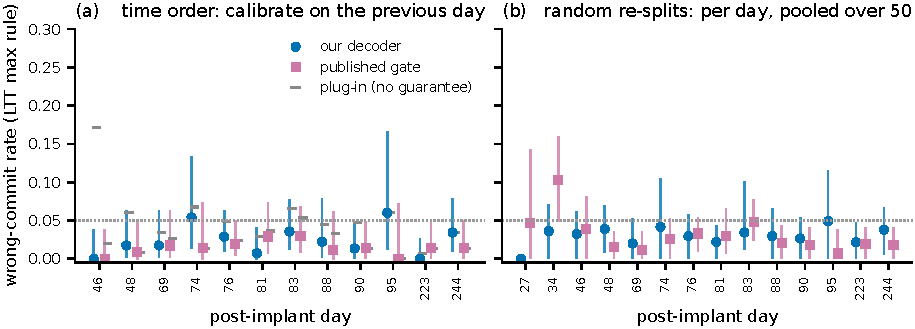
\includegraphics[width=\linewidth]{fig_deploy.pdf}
  \caption{\textbf{The guaranteed rule across days} (Brain-to-Text '25, guard on, LTT max rule; dotted line: $\alpha = 0.05$). (a)~Time order (V1: fit on days $1..k{-}2$, calibrate on day $k{-}1$, test on day $k$): wrong-commit rate per test day with exact CP 95\% CIs; small grey markers: plug-in rule. (b)~Random re-splits: wrong-commit rate per day pooled over 50 re-splits; bars: 5th--95th percentile over re-splits. The bound covers the mix of days; on the published gate, day 34 ran at about $2\alpha$.}
  \label{fig:deploy}
\end{figure}

\subsection{Random re-splits and the scope of the guarantee}
\label{sec:res-resplits}
\label{sec:res-perday}
Over 50 random re-splits (\cref{tab:repeat}), the LTT max rule gave mean wrong-commit rates of 0.030 (our decoder) and 0.031 (published gate). It exceeded $\alpha$ on the test set in 4/50 = 0.08 \ci{0.02}{0.19} and 1/50 = 0.02 \ci{0.001}{0.11} of re-splits. Fifty re-splits cannot show that this share is at most $\delta = 0.1$, and the test-set share includes test-sampling noise. The exact population exceedance, which LTT bounds, was 0.026 and 0.014. CRC met its own target, the mean (0.046 and 0.049), and, as designed, many single re-splits were above $\alpha$ (34\% and 42\%). LTT max was never above $\alpha$ in a re-split where CRC max was not; with 50 re-splits this difference was significant only on the published gate (exact McNemar $p = 0.25$ and $0.031$; with 200 re-splits $p < 10^{-6}$ on both, \cref{app:population}). With the guard off, LTT max exceeded $\alpha$ in 0 of 50 re-splits on both decoders. On sEMG, LTT max committed 9\% and 2\% of sentences (session-calibrated, cross-session; mean wrong-commit 0.011 and 0.006) and never exceeded $\alpha$; on cross-session, 34\% of re-splits never committed, and the cross-subject decoder never committed.

Per day, the risk was not controlled (\cref{fig:deploy}b, \cref{tab:perday}). On the published gate, day 34 (about 50 test trials per re-split) had a pooled wrong-commit rate of 0.102 under LTT max, and it was above $\alpha$ in 94\% of re-splits; in fixed splits A and B it had 8 wrong commits in 50 trials (0.16, CP95 \ci{0.07}{0.29}). The other days had 0.007--0.048, and our decoder 0.000--0.049 on every day. LTT bounds the risk over the mix of days that the calibration set comes from, not each day. Per-day (Mondrian) LTT with a quarter of each day as calibration was feasible only on the one day with at least 45 calibration items, and committed nothing on the other 13 days.

The guaranteed rule was faster than the same fitted policy without commits in every re-split: by $+0.114$ \ewpm{} (Monte-Carlo SE 0.005) on our decoder and $+0.510$ (SE 0.007) on the published gate, about 1\% and 3\%. On the fixed test set, the paired gains were $+0.058$ \ci{0.034}{0.090} and $+0.125$ \ci{0.077}{0.188} (ours, splits A and B) and $+0.537$ \ci{0.439}{0.636} and $+0.567$ \ci{0.456}{0.694} (published).

\begin{table}[t]
  \centering
  \caption{\textbf{Random re-splits} (50; exchangeable by construction, so a check of the theorems on one data pool, not a deployment test). Wrong-commit: mean test rate (5th--95th percentile over re-splits); $>\alpha$: share of re-splits with a test rate above $\alpha$, with exact CP 95\% CI; Pop.: share of with-replacement calibration draws whose exact population risk exceeds $\alpha$ (\cref{app:population}); Commit: mean; EAC: pooled; Gain: mean paired \ewpm{} gain over the same fitted policy without commits. The spread is split-to-split variation in one data set, not a CI for new data. sEMG rows: \cref{tab:repeat-full}.}
  \label{tab:repeat}
  \small
  \begin{adjustbox}{max width=\linewidth}\begin{tabular}{@{}lllllll@{}}
    \toprule
    \textbf{Rule} & \textbf{Wrong-commit} & $\boldsymbol{>\alpha}$ \textbf{[CP95]} & \textbf{Pop.} & \textbf{Commit} & \textbf{EAC} & \textbf{Gain} \\
    \midrule
    \multicolumn{7}{@{}l}{\textit{Brain-to-Text '25, our decoder}} \\
    plug-in (fit-A) & 0.044 (0.021--0.072) & 0.34 \ci{0.21}{0.49} & --- & 0.19 & 0.24 & $+0.132$ \\
    CRC, pure & 0.046 (0.026--0.068) & 0.34 \ci{0.21}{0.49} & 0.39 & 0.19 & 0.24 & --- \\
    CRC, max rule & 0.037 (0.021--0.059) & 0.14 \ci{0.06}{0.27} & 0.17 & 0.17 & 0.22 & $+0.125$ \\
    \textbf{LTT, max rule} & \textbf{0.030} (0.016--0.052) & \textbf{0.08} \ci{0.02}{0.19} & 0.026 & 0.15 & 0.21 & $+0.114$ \\
    LTT, max rule, guard off & 0.031 (0.013--0.043) & 0.00 \ci{0}{0.07} & --- & 0.14 & 0.21 & $+0.106$ \\
    \midrule
    \multicolumn{7}{@{}l}{\textit{Brain-to-Text '25, published gate}} \\
    plug-in (fit-A) & 0.039 (0.021--0.060) & 0.22 \ci{0.12}{0.36} & --- & 0.43 & 0.09 & $+0.564$ \\
    CRC, pure & 0.049 (0.029--0.075) & 0.42 \ci{0.28}{0.57} & 0.40 & 0.48 & 0.10 & --- \\
    CRC, max rule & 0.036 (0.021--0.055) & 0.14 \ci{0.06}{0.27} & 0.074 & 0.42 & 0.09 & $+0.546$ \\
    \textbf{LTT, max rule} & \textbf{0.031} (0.020--0.047) & \textbf{0.02} \ci{0.001}{0.11} & 0.014 & 0.39 & 0.08 & $+0.510$ \\
    LTT, max rule, guard off & 0.024 (0.018--0.031) & 0.00 \ci{0}{0.07} & --- & 0.36 & 0.07 & $+0.471$ \\
    \bottomrule
  \end{tabular}\end{adjustbox}
\end{table}

\subsection{Fixed test sets; sEMG and MEG as format and safety checks}
\label{sec:res-main}
On the fixed test set (\cref{tab:main}), always committing sent wrong text for 0.610 of trials on our decoder and 0.194 on the published sentence, because one wrong word makes a sentence wrong. The guaranteed rule gave 0.025 and 0.052 (splits A and B) on our decoder and 0.029 and 0.031 on the published gate. The plug-in layer fitted on all fit trials gave 0.059 \ci{0.045}{0.070} on our decoder, above $\alpha$. The difference to the fit-A rows comes from the policy grid fitted on fit-A, not from the risk control: in split A, CRC and LTT were not binding (\cref{app:full}). On sEMG, the layer cut the wrong-commit rate from 0.541, 0.882 and 0.962 to 0.004, 0.004 and 0, committing 21, 10 and 0 of 551 sentences; the guaranteed rule gave the same rows. On MEG the layer committed nothing (0 of 637, one-sided 95\% upper bound 0.0047) and equals always offering; no guarantee for new sentences is possible on these data, because a sentence-level LTT needs at least 45 calibration sentences and the data set has 17 test sentences (\cref{app:meg}). Only the session-calibrated sEMG decoder clearly beat gaze typing \ci{+2.71}{+4.91}; on the 256 sEMG test sentences without a near variant in the LM text, speeds were lower and gaze typing beat the cross-subject decoder (\cref{app:leakage}).

\begin{table}[t]
  \centering
  \caption{\textbf{Safety and speed on the fixed test sets.} Plug-in: full fit, no guarantee. Guaranteed rule (the frozen configuration of \cref{sec:discussion}): fit-A pipeline, guard, clean calibration, LTT max rule (B2T '25: splits A and B, $n_{\mathrm{cal}} = 401$; sEMG: 143). Guard off: the same with the plain threshold. EAC: error among commits (wrong/commits in brackets; count only if fewer than 30 commits). Silent: uncorrected wrong final texts per item. 95\% cluster-bootstrap CIs over days (B2T '25), participants (sEMG) or sentences $\times$ participants (MEG), conditional on the fitted pipeline and threshold. Zero rates: one-sided 95\% upper bounds 0.0037 (816 items), 0.0054 (551) and 0.0047 (637). All policies: \cref{tab:full}.}
  \label{tab:main}
  \small
  \begin{adjustbox}{max width=\linewidth}\begin{tabular}{@{}lllllll@{}}
    \toprule
    \textbf{Device} & \textbf{Policy} & \textbf{\ewpm{} [CI]} & \textbf{Wrong-commit [CI]} & \textbf{Commit} & \textbf{EAC} & \textbf{Silent} \\
    \midrule
    B2T '25, our decoder & always commit & 11.45 \ci{10.70}{12.31} & 0.610 \ci{0.568}{0.647} & 1.00 & 0.61 & 0.044 \\
     & always offer & 11.37 \ci{10.67}{12.17} & 0 & 0 & --- & 0 \\
     & plug-in & 11.55 \ci{10.83}{12.34} & 0.059 \ci{0.045}{0.070} & 0.23 & 0.25 (48/189) & 0.003 \\
     & \textbf{guaranteed rule, A} & 11.48 \ci{10.79}{12.29} & \textbf{0.025} \ci{0.015}{0.035} & 0.10 & 0.24 (20/82) & 0.001 \\
     & \textbf{guaranteed rule, B} & 11.54 \ci{10.83}{12.34} & \textbf{0.052} \ci{0.043}{0.059} & 0.19 & 0.27 (42/157) & 0.003 \\
     & guard off, A & 11.55 \ci{10.83}{12.39} & 0.040 \ci{0.030}{0.051} & 0.18 & 0.22 (33/149) & 0 \\
     & guard off, B & 11.53 \ci{10.82}{12.37} & 0.029 \ci{0.021}{0.038} & 0.15 & 0.20 (24/120) & 0 \\
    B2T '25, published & always commit & 19.61 \ci{17.81}{21.32} & 0.194 \ci{0.146}{0.253} & 1.00 & 0.19 & 0.025 \\
     & always offer & 18.11 \ci{16.59}{19.57} & 0 & 0 & --- & 0 \\
     & plug-in & 18.77 \ci{17.13}{20.35} & 0.044 \ci{0.027}{0.068} & 0.47 & 0.09 (36/386) & 0.004 \\
     & \textbf{guaranteed rule, A} & 18.65 \ci{17.04}{20.20} & \textbf{0.029} \ci{0.013}{0.050} & 0.40 & 0.07 (24/329) & 0.001 \\
     & \textbf{guaranteed rule, B} & 18.68 \ci{17.06}{20.23} & \textbf{0.031} \ci{0.014}{0.052} & 0.42 & 0.07 (25/339) & 0.003 \\
     & guard off, A & 18.63 \ci{17.03}{20.18} & 0.027 \ci{0.016}{0.040} & 0.39 & 0.07 (22/319) & 0.001 \\
     & guard off, B & 18.63 \ci{17.02}{20.18} & 0.025 \ci{0.014}{0.038} & 0.39 & 0.06 (20/316) & 0.001 \\
    B2T '25 & gaze typing & 4.08 \ci{4.05}{4.12} & 0 & --- & --- & 0 \\
    \midrule
    sEMG session-cal. & always commit & 7.81 \ci{6.66}{9.04} & 0.541 \ci{0.463}{0.621} & 1.00 & 0.54 & 0.060 \\
     & \textbf{guaranteed rule} & 7.98 \ci{6.95}{9.11} & \textbf{0.004} \ci{0}{0.009} & 0.04 & 2/21 & 0 \\
    sEMG cross-session & always commit & 4.10 \ci{3.56}{4.73} & 0.882 \ci{0.831}{0.928} & 1.00 & 0.88 & 0.149 \\
     & \textbf{guaranteed rule} & 4.68 \ci{4.19}{5.25} & \textbf{0.004} \ci{0}{0.009} & 0.02 & 2/10 & 0 \\
    sEMG cross-subject & always commit & 3.53 \ci{3.19}{3.90} & 0.962 \ci{0.942}{0.981} & 1.00 & 0.96 & 0.167 \\
     & \textbf{guaranteed rule} & 4.08 \ci{3.82}{4.37} & \textbf{0} & 0 & --- & 0 \\
    sEMG & gaze typing & 4.27 \ci{4.22}{4.32} & 0 & --- & --- & 0 \\
    \midrule
    MEG (asynchronous) & always commit & 2.58 \ci{2.31}{2.88} & 0.997 \ci{0.987}{1.000} & 1.00 & 1.00 & 0.235 \\
     & trust (= always offer) & 3.20 \ci{3.01}{3.44} & 0 & 0 & --- & 0 \\
    MEG & gaze typing & 3.15 \ci{3.02}{3.31} & 0 & --- & --- & 0 \\
    \bottomrule
  \end{tabular}\end{adjustbox}
\end{table}

\subsection{A guaranteed error among commits of 10\% almost never commits}
\label{sec:res-selective}
The marginal rules let a weak decoder commit text that is often wrong: 21\% of the guaranteed rule's commits on our decoder (\cref{tab:repeat}). Joint LTT bounds both risks (\cref{tab:selective}). With $\beta = 0.10$ it committed nothing on our decoder, sEMG and MEG, nothing in either fixed split, and nothing in any time-ordered design with one day of calibration. Over random re-splits of the published gate, it committed 7.2\% of sentences on average (none in 76\% of re-splits), with an error among commits of 0.059. With $\beta = 0.20$, it committed 32\% of published sentences with an error among commits of 0.062, and 0.32 in fixed split A (error among commits 0.057 \ci{0.032}{0.093}); our decoder still committed 0.1\%. LTT-sel, which bounds only the selective risk, committed 56\% of published sentences at $\beta = 0.20$, but its marginal rate (0.074) exceeded $\alpha$ in 76\% of re-splits. The limit is the calibration size: an exact bound on the error among commits needs many calibration commits.

\begin{table}[t]
  \centering
  \caption{\textbf{Controlling the error among commits} (B2T '25 published gate, 50 random re-splits, guard on, $\delta = 0.1$; test set). Commit: mean (share of re-splits with no commit); EAC: pooled error among commits; $>\beta$: committing re-splits with EAC above $\beta$; Marginal: mean wrong-commit rate ($>\alpha$: share of re-splits above $\alpha$). Joint LTT: both targets, fixed grid, Bonferroni (valid for both). LTT-sel: selective target only. SGR: bisection \citep{geifman2017selective}. Our decoder: joint LTT commits nothing at $\beta = 0.10$ and 0.1\% at $\beta = 0.20$; sEMG and MEG: no commits at any $\beta$.}
  \label{tab:selective}
  \small
  \begin{adjustbox}{max width=\linewidth}\begin{tabular}{@{}llllllll@{}}
    \toprule
    $\boldsymbol\beta$ & \textbf{Rule} & \textbf{Commit (none)} & \textbf{EAC} & $\boldsymbol{>\beta}$ & \textbf{Marginal} & $\boldsymbol{>\alpha}$ & \textbf{\ewpm{}} \\
    \midrule
    0.10 & \textbf{joint LTT} & 0.072 (0.76) & 0.059 & 0 of 12 & 0.004 & 0 & 18.07 \\
         & LTT-sel & 0.072 (0.76) & 0.059 & 0 of 12 & 0.004 & 0 & 18.07 \\
         & SGR & 0.112 (0.64) & 0.069 & 0 of 18 & 0.008 & 0 & 18.12 \\
    0.20 & \textbf{joint LTT} & 0.318 (0.02) & 0.062 & 0 of 49 & 0.020 & 0 & 18.39 \\
         & LTT-sel & 0.564 (0) & 0.131 & 0 of 50 & 0.074 & 0.76 & 18.72 \\
         & SGR & 0.617 (0) & 0.142 & 0 of 50 & 0.088 & 0.92 & 18.79 \\
    --- & LTT max rule (marginal only) & 0.392 (0) & 0.078 & --- & 0.031 & 0.02 & 18.49 \\
    --- & no commits & 0 (1) & --- & --- & 0 & 0 & 17.98 \\
    \bottomrule
  \end{tabular}\end{adjustbox}
\end{table}

\subsection{Controls: without the guard, the layer commits no-information streams}
\label{sec:res-null}
Always committing wrote a sentence for every control stream. With the guard, the guaranteed rule (split A) committed none of the 300 frame-shuffled and none of the 300 uniform streams on either Brain-to-Text '25 decoder (one-sided 95\% upper bound 0.0099), while it committed 29 (ours) and 115 (published) of the 300 matched real trials; the full-fit layer also committed none, and so did sEMG (0 of 200 sentences per control; bound 0.015) (\cref{fig:null}). Without the guard, our decoder committed 198 of 300 uniform streams under the plain threshold with the LTT max rule (all 198 commits wrong) and 3 of 300 frame-shuffled streams. A uniform stream gives flat phoneme posteriors; the word decoder then returns a fluent LM sentence with a high calibrated $\hat p_{\mathrm{top1}}$, and the calibration data, which contain only real streams, cannot detect this. The published gate, sEMG and MEG committed no control stream with or without the guard. On real data, in contrast, the guard did not lower wrong commits. Without it, the full-fit wrong-commit rate on our decoder fell from 0.059 to 0.036 (paired \ci{-0.035}{-0.011}; sign test over days $p = 0.021$). In the re-splits, the time-ordered tests and the fixed splits, the rates without the guard were lower on the published gate in 6 of 7 comparisons and mixed on our decoder (lower in 2, similar in 2, higher in 3; fixed split A: 0.040 against 0.025) (\cref{tab:repeat,tab:main,tab:forward-full}). A commit rule therefore needs an input-validity check that real calibration data do not test; in these fits our guard was one such check, but not in every fit: the grid value $r_{\max} = 1.0$ switches its limit off (\cref{app:guardlimit}). A better check is open. Given the real stream of another sentence (intent mismatch), the layer committed at the matched rate on our decoder: nothing in the stream reveals the intent. The published gate committed none of these 300 streams (\cref{tab:controls}).

\subsection{Speed depends on the user model; wrong-commit rates do not}
\label{sec:res-user}
\Cref{fig:usermodel} refits every policy (plug-in layer) under eight user-model variants. The layer was at least as fast as always offering in every variant and condition. Always committing was faster than the layer on the published gate in all 9 variants (by 0.46--1.47 \ewpm{}, every CI below 0) and on our decoder in 5 of 9 (CI below 0 in 1, above 0 in 3). Gaze typing with word completion had a higher point value than the layer in every variant on MEG and on the two weaker sEMG decoders. The wrong-commit rate of the refitted layer was at most 0.059 in all 54 condition--variant pairs.

\begin{figure}[t]
  \centering
  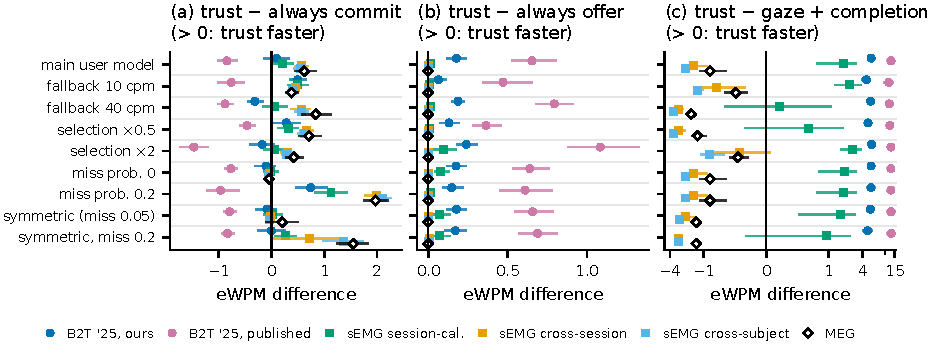
\includegraphics[width=\linewidth]{fig_user_model.pdf}
  \caption{\textbf{User-model sensitivity} (plug-in layer, full fit; not the guaranteed rule). Paired \ewpm{} difference between the trust layer and (a)~always committing, (b)~always offering and (c)~gaze typing with word completion (symmetric-log axis), all policies refitted under each variant (rows); values above 0 mean that the layer is faster. 95\% cluster-bootstrap CIs at the primary unit.}
  \label{fig:usermodel}
\end{figure}

\subsection{Calibration and the other components}
\label{sec:res-ablation}
Sentence ECE fell from 0.448 \ci{0.419}{0.475} to 0.067 \ci{0.065}{0.104} on our intracortical decoder and from 0.102 \ci{0.058}{0.161} to 0.058 \ci{0.044}{0.090} on the published gate (percentile CIs; binned ECE is biased upwards, so an interval can lie beside its point value). The calibrated $\hat p_{\mathrm{top1}}$ predicted a wrong top sentence with AUROC 0.797 \ci{0.773}{0.819} (ours), 0.710 \ci{0.678}{0.744} (published) and 0.828, 0.755 and 0.674 on sEMG (\cref{app:ece}); the MEG AUROC is not informative (2 right sentences). The frame temperature raised the ECE of per-frame phoneme peaks (0.090 to 0.130) although it minimises their cross-entropy; we did not resolve why, but the two criteria differ (cross-entropy at aligned peaks with blank targets for inserted peaks, ECE of the arg-max confidence). Without the sentence temperature, wrong commits rose on 4 of 6 conditions (\cref{tab:ablation}). Calibrating pure CRC on data that had also fitted the pipeline raised the test rate on our decoder by $+0.009$ (day-jackknife 95\% CI \ci{+0.005}{+0.013}; Holm-adjusted $p = 0.004$ over 12 comparisons), conditional on this data pool; no other condition showed an effect after Holm, and with 200 re-splits the effect was $+0.003$ (\cref{tab:reuse}). As the threshold varies, the published decoder can commit about half of its sentences at the 0.05 marginal level and our decoder about a fifth (\cref{fig:calib}).

\section{Discussion}
\label{sec:discussion}

\paragraph{The layer is a safety mechanism, tested on one person.} All non-trivial evidence for the commit decision comes from one intracortical participant in a copy task. On that participant, a stream-level rule with a high-probability guarantee kept the wrong-commit rate below 5\% when it was calibrated on earlier days and tested on later ones, and in random re-splits of the same data. It was faster than the same policy without commits by about 1\% and 3\%, which is within the uncertainty of the user model, and it was slower than always committing for the published decoder. On sEMG and MEG the layer reduced to always offering, the correct behaviour for decoders whose top sentence was rarely right; it cannot create information that the decoder lacks.

\paragraph{Which guarantee to deploy, and for which unit.} CRC met its target as a mean, as it promises, but a third or more of single calibration sets exceeded $\alpha$. LTT bounds the risk of the calibration distribution with high probability, at almost no speed cost against CRC with the max rule. That distribution is a mixture of sessions. On the published gate, one day in 14 ran at about $2\alpha$ under LTT, and a user meets one session at a time. The deployable statement is therefore ``at most 5\% wrong commits over the mix of sessions that the calibration data represent'', with its assumptions, its unit and the measured silent-error rate (\cref{app:guarantees}). Per-session control needs per-session calibration: with LTT at least 45 calibration sentences per session, which is a long session-start block for a BCI user, or a group-conditional method that pools strength across sessions. In our time-ordered tests, a session-start block of half a day kept the pooled rate at 0.010--0.015 but did not remove the high day.

\paragraph{Who sets $\alpha$ and $\beta$.} The marginal wrong-commit rate is the budget of harm per sentence attempted; the error among commits is what a user sees in committed text. With current decoders the two diverge: one in five commits of the guaranteed rule on our decoder was wrong, and a user who sees this will learn to check every commit, which turns commits into offers. A valid joint bound with $\beta = 0.10$ almost never committed with a few hundred calibration sentences; $\beta = 0.20$ was usable only on the published gate. Potential BCI users asked for at least 90\% accuracy \citep{huggins2011als,huggins2015sci}; they were asked about accuracy in general, and our reading that this suggests $\beta \le 0.10$ for committed sentences is an interpretation. The targets should be chosen by the user with their clinician and communication partners, and may differ by context. Our exact-match loss treats a harmless near miss like a meaning-changing error; a loss weighted by semantic severity, scored by users, is the natural next target. Conformal selection with false-discovery-rate control \citep{jin2023selection,gui2024alignment} bounds the expected error among commits and may commit more at the same $\beta$; it is the natural comparator to test next.

\paragraph{A commit rule needs an input-validity check.} Calibration data contain real streams only, so a guarantee calibrated on them says nothing about streams that carry no neural information. Our plain threshold committed most uniform streams on our decoder, because its LM turns flat posteriors into fluent sentences with high calibrated confidence. The guard stopped this, but it did not lower wrong commits on real data, and with the full-fit pipeline it raised them. A deployed system needs a separate check that the input carries evidence, tested on signal-destroying controls.

\paragraph{Strong decoders still need a gate.} The published decoder has a WER of 0.043, yet 19\% of its sentences were wrong. Gating its text by agreement with a light reference decoder on the same stream kept 95\% of the always-commit \ewpm{} under the main user model (18.65 vs 19.61, fixed split A) and reduced wrong commits from 19\% to 2.9\%. This needs the stream and a reference decoder; the published text alone gave no usable confidence.

\paragraph{A frozen configuration for a confirmatory test.} All analyses, including those that shaped the method, used the same Brain-to-Text '25 data, so all results here are exploratory. For a confirmatory test on data we have not used (a second participant, or new sessions), we fix this configuration: frame and sentence temperatures; the guard as in \cref{tab:settings}; the policy grid of \cref{app:settings} fitted on fit-A; LTT with the max rule on a disjoint calibration set that precedes the test data in time; $\alpha = 0.05$, $\delta = 0.1$; joint LTT with $\beta = 0.10$ and $0.20$ as secondary rules. The primary outcomes are the pooled and per-session wrong-commit rates, the error among commits and the commit rate on the signal-destroying controls. This configuration is tagged \code{paper1-v4-frozen-config} in the repository; later commits changed only the manuscript text. It replaces the tag \code{paper1-v3-frozen-config} (commit \code{65359dc}), which froze the plain threshold without the guard; that configuration failed the no-information control (\cref{sec:res-null}), so it must not be used. We keep the old tag for the record.

\section{Limitations}
\label{sec:limitations}

\begin{enumerate}[leftmargin=*,itemsep=0pt]
  \item \textbf{One implant participant} in a copy task, with online logits we cannot re-run, is the only non-trivial test of the commit decision. Our intervals cover days and splits of this person, not people. The time-ordered test has 10--13 test days, too few to confirm per-day control. Two pre-registered confirmatory tests on a second participant (T12, Brain-to-Text '24, CC0) were uninformative: the frozen configuration committed 0 and 1 of 400 test trials, below the pre-registered informative conditions (at least 1 and at least 21 commits). They had no wrong commits and the controls passed, but the cause was our weak decoder (test PER 0.54, then 0.27) with the strict fitted guard limit, so the bound still rests on one participant (\cref{app:t12}).
  \item \textbf{The guarantee covers the mix of sessions}, not each session; one day ran at about $2\alpha$. All guarantees count only observed errors, and stream-level gating cannot detect intent mismatch.
  \item \textbf{The input-validity check} that made the layer safe on no-information streams in the reported fits (the guard) did not lower wrong commits on real data (it raised them with the full-fit pipeline), and it was tested on synthetic controls only. The fitted grid value $r_{\max} = 1.0$ switches it off (\cref{app:guardlimit}).
  \item \textbf{Composed sEMG sentences and a weak MEG decoder}: isolated presses with oracle timing and templated test sentences (295 of 551 with a near variant in the LM text); 17 unique MEG test sentences, too few for a sentence-level guarantee.
  \item \textbf{No live users.} Only two user costs are measured, in one gaze-typing user; speed rankings change across plausible variants; the word-completion baseline is weaker than clinical AAC; the loss is exact match. A user study needs ethics approval.
\end{enumerate}

\section{Conclusion}
\label{sec:conclusion}

A trust layer on a per-frame output stream can decide whether a neural text-entry decoder commits, offers or abstains, with a high-probability bound on the wrong-commit rate. On one intracortical participant, Learn-then-Test with the max rule kept wrong commits below 5\% when calibrated on earlier days and tested on later ones, but the bound covers the mix of sessions, not each session. About one in five (our decoder) or one in thirteen (published decoder) committed sentences was still wrong, and a valid bound on the error among commits almost never committed. Without an input-validity check, the layer committed no-information streams. Next steps are a confirmatory test of the frozen configuration on new data, per-session calibration, and a user study of which error rates users accept.

\section*{Ethics, data and code availability}
\label{sec:ethics}
\label{sec:availability}

This study is a secondary analysis of publicly available, de-identified data sets that their original investigators released under public licences: Brain-to-Text '25 (BrainGate2, ClinicalTrials.gov NCT00912041; CC0 \citep{card2025data}), Toronto sEMG typing (CC BY 4.0 \citep{achituve2024data}) and SpanishBCBL MEG (CC BY-NC 4.0 \citep{spanishbcbl}). No new data were collected and no experiment with human participants was run. The original studies report their ethics procedures in their publications: the intracortical data come from participant T15 of the BrainGate2 clinical trial, collected under that trial's consent and institutional review board approval \citep{card2024accurate}; the MEG study was approved by the local ethics committee and its participants gave informed consent \citep{levy2026brain2qwerty}; the sEMG data set and its collection are described in its data descriptor \citep{achituve2025emg}. No further approval was required for this secondary analysis. From Brain-to-Text '25 we use only the logits, cue sentences and published sentences. We did not attempt re-identification of any participant. Quoted sentences are public copy-task cues, not the participant's own words. No raw recordings or participant data are redistributed (data sets and licences: \cref{tab:licences}).

The \nts{} specification, conformance suite, reference implementation and all experiment scripts are at \url{https://github.com/zhangzibo/fidetype} (Apache-2.0), without weights trained on SpanishBCBL or copied Brain2Qwerty code. Every table and figure is generated from committed result files by committed scripts. The per-split item tables are derived numbers (no signals or texts) kept in a local cache; they can be rebuilt with the committed commands. The version of the code used for this paper is tagged \code{paper1-v4-frozen-config} in that repository. This article is distributed under the Creative Commons Attribution 4.0 International licence (CC BY 4.0). The trust layer took a median of 0.18--0.30\,ms per decision on one CPU thread (95th percentile at most 1.06\,ms), against 45--232\,ms for the beam-search decoders.


\section*{Funding}
This work received no specific funding.

\section*{Competing interests}
The author declares no competing interests.

\section*{Use of AI assistance}
Code, analyses and manuscript drafting were carried out with substantial assistance from an AI system (Claude, Anthropic). The author directed the work, reviewed the results and takes full responsibility for the content. All numbers come from committed scripts and result files.

\bibliographystyle{unsrtnat}
\bibliography{main}

\appendix
\section{Trust decision and main user model}
\label{app:algorithm}

Algorithm~\ref{alg:decide} is the decision for one item; Algorithm~\ref{alg:calibrate} (supplement) gives the fitting and calibration. The reference implementation is \code{fidetype.trust} and \code{fidetype.eval.harness}. \Cref{tab:user} lists the main simulated user; only the first two values are measured \citep{cai2024gaze}.

\begin{algorithm}[H]
\caption{Trust decision for one item}
\label{alg:decide}
\small
\begin{algorithmic}[1]
\Require stream $\log p_t(v)$, $t = 1..F$; fitted $\tau_f, \tau_s, q$; policy $(\lambda, r_{\max}, r_{\mathrm{abst}}, k_{\max}, \text{fallback})$
\State $\tilde\ell_t(v) \gets \log p_t(v)/\tau_f - \log\sum_{u} p_t(u)^{1/\tau_f}$ \Comment{frame calibration, before the LM}
\State $(y_1..y_K, \text{score}_1..\text{score}_K) \gets$ CTC prefix beam search with LM on $\tilde\ell$ \Comment{$K$-best list}
\If{the list is empty} \Return \act{abstain}
\EndIf
\State $\hat p_j \gets \mathrm{softmax}_j(\text{score}/\tau_s)$; \quad $\hat p_{\mathrm{top1}} \gets \hat p_1$
\State $C \gets \{\, j : 1 - \hat p_j \le q \,\}$, ordered by $\hat p_j$ \Comment{conformal sentence set}
\For{each character $m$ of $y_1$} \Comment{acoustic confidence}
  \State char streams: $a_m \gets \max_{t \in \mathrm{span}(m)} \exp\tilde\ell_t(y_{1,m})$ (CTC forced alignment of $y_1$)
  \State phoneme path: $a_m \gets 0.5^{e}\min_{\text{phonemes of the word}} \exp\tilde\ell$ at their peak frames ($e$ = lexicon edits)
\EndFor
\State $\mathrm{low} \gets \frac{1}{|y_1|}\#\{m : a_m < 0.5\}$ \Comment{low-evidence share}
\State $\mathrm{cons} \gets \sum_{j \le 5} \hat p_j\, \mathrm{sim}(y_1, y_j) / \sum_{j \le 5} \hat p_j$, \quad $\mathrm{sim}(a,b) = 1 - \mathrm{WED}(a,b)/\max(|a|_w, |b|_w)$
\State $g \gets \min\bigl(1, \max(\mathrm{low},\, 1 - \mathrm{cons})\bigr)$ \Comment{guard risk; WED = word edit distance}
\If{$g \ge r_{\mathrm{abst}}$} \Return \act{abstain}
\EndIf
\State $s \gets \hat p_{\mathrm{top1}}$ if $g \le r_{\max}$ else $-\infty$ \Comment{commit score}
\If{$s \ge \lambda$} \Return \act{commit} $y_1$
\EndIf
\If{$1 \le |C| \le k_{\max}$ and $C$ does not contain the ``other'' option} \Return \act{offer} $C$
\EndIf
\State \Return \act{offer} $y_1..y_{k_{\max}}$ if fallback = offer and $k_{\max} \ge 1$, else \act{abstain}
\end{algorithmic}
\end{algorithm}

\begin{table}[H]
  \centering
  \caption{\textbf{Main simulated-user parameters.} Variants: \cref{app:user}.}
  \label{tab:user}
  \small
  \begin{adjustbox}{max width=\linewidth}\begin{tabular}{@{}lll@{}}
    \toprule
    \textbf{Parameter} & \textbf{Value} & \textbf{Basis} \\
    \midrule
    Fallback (gaze keyboard) speed & 20 characters/min & measured, eye-gaze user LP1 \citep{cai2024gaze} \\
    Scan and select one of $k$ word alternatives & $1.0 + 1.0\log_2(k+1) + 1.5$\,s (4.5\,s for $k = 3$) & sum close to the measured 4.7\,s \citep{cai2024gaze} \\
    Select one of $k$ offered sentences & $1.0 + 0.5\log_2(k+1)$\,s & assumption \\
    Reading time & 0.3\,s per word, 0.5\,s per candidate & assumption \\
    Navigate to and delete a wrong word & 3.0\,s (2 selections) & assumption \\
    Miss probability of a wrong, unmarked word after a commit & 0.05 & assumption (no measurement) \\
    Errors in offered candidates & always seen (main model) & assumption \\
    Full retype overhead & 1.5\,s; chosen when cheaper than fixing words & assumption (rational user) \\
    Abstain overhead & 0.5\,s, then fallback typing & assumption \\
    Neural input speed, MEG / B2T '25 / sEMG & 152 / 159.3 / 75.8 characters/min & device setting \\
    \bottomrule
  \end{tabular}\end{adjustbox}
\end{table}


% ---------------------------------------------------------------- supplementary material
\clearpage
\setcounter{section}{0}
\setcounter{table}{0}
\setcounter{figure}{0}
\setcounter{algorithm}{0}
\setcounter{equation}{0}
\renewcommand{\thesection}{S\arabic{section}}
\renewcommand{\thetable}{S\arabic{table}}
\renewcommand{\thefigure}{S\arabic{figure}}
\renewcommand{\thealgorithm}{S\arabic{algorithm}}
\renewcommand{\theequation}{S\arabic{equation}}
% unique hyperref anchors for the S-numbered objects
\renewcommand{\theHsection}{S\arabic{section}}
\renewcommand{\theHtable}{S\arabic{table}}
\renewcommand{\theHfigure}{S\arabic{figure}}
\providecommand{\theHalgorithm}{}\renewcommand{\theHalgorithm}{S\arabic{algorithm}}
\renewcommand{\theHequation}{S\arabic{equation}}
% S-sections are "Section S1", not "Appendix S1" (undo the \appendix switch of cleveref)
\crefalias{appendix}{section}
\crefalias{subappendix}{subsection}

\begin{center}
  {\Large\bfseries Supplementary material}
\end{center}
\noindent The supplementary material follows. Its sections, tables, figures, algorithms and equations carry the prefix S. Sections 1--9, Tables 1--5, Figures 1--3, Algorithm 1 and Appendix A are in the main text above. All numbers come from committed result files and scripts in the repository (\url{https://github.com/zhangzibo/fidetype}).
\addcontentsline{toc}{section}{Supplementary material}

% Supplementary material of Paper 1. Section, table, figure and algorithm numbers carry the prefix S.
% References to the main paper (sections, Tables 1-4, Figures 1-3, Algorithm 1) resolve through xr (main.aux).

\section{Notation}
\label{app:notation}

\begin{table}[H]
  \centering
  \caption{\textbf{Notation.} Prose uses ``error among commits''; tables use EAC.}
  \label{tab:notation}
  \small
  \begin{adjustbox}{max width=\linewidth}\begin{tabular}{@{}ll@{\qquad}ll@{}}
    \toprule
    \textbf{Symbol} & \textbf{Meaning} & \textbf{Symbol} & \textbf{Meaning} \\
    \midrule
    $F_i$, $V$ & frames in the stream of item $i$; vocabulary size & $\lambda$ & commit threshold on $s_i$ \\
    $K$ & candidate list size ($K = 10$; 11 for the published gate) & $s_i$ & commit score: $\hat p_{\mathrm{top1}}$ if eligible, else $-\infty$ \\
    $\hat p_{\mathrm{top1}}$ & calibrated probability of the top candidate & $c_i$ & 1 if the top candidate is wrong \\
    $\tau_f$, $\tau_s$ & frame and sentence temperatures & $L_i(\lambda)$ & loss $c_i\,\mathbf{1}[s_i \ge \lambda]$ \\
    $g_i$ & guard risk of the top candidate, in $[0,1]$ & $R(\lambda)$, $\hat R_n(\lambda)$ & population and calibration risk \\
    $r_{\mathrm{abst}}$, $r_{\mathrm{max}}$ & guard limits for abstain and commit & $n$ & number of calibration items \\
    $k$, $k_{\max}$ & offered candidates; offer limit & $\alpha$ & target wrong-commit rate (0.05) \\
    $q$ & conformal quantile of the sentence set & $\beta$ & target error among commits (0.10, 0.20) \\
    $n_\lambda$, $k_\lambda$ & calibration commits and wrong commits at $\lambda$ & $\delta$ & failure probability of LTT (0.1) \\
    $\eta$, $\gamma$ & step sizes of the online controllers & $T$, $d$ & items in an online sequence; feedback delay \\
    \bottomrule
  \end{tabular}\end{adjustbox}
\end{table}

\section{Fitting and calibration}
\label{app:algorithms}

\begin{algorithm}[H]
\caption{Fitting and calibration of the commit threshold}
\label{alg:calibrate}
\small
\begin{algorithmic}[1]
\Require fit items $\mathcal{F}$ (parts $\mathcal{F}_1$, $\mathcal{F}_2$, $\mathcal{F}_3$; see below), disjoint calibration items $\mathcal{C}$ ($n$ items with truth), $\alpha$, $\beta$, $\delta$
\State $\tau_f \gets \arg\min_\tau$ cross-entropy of the aligned true tokens at the greedy CTC peaks of $\mathcal{F}_1$ \Comment{golden section, $\tau \in [0.05, 20]$}
\State $\tau_s \gets \arg\min_\tau$ binary NLL of $[y_1 = \text{truth}]$ under $\mathrm{softmax}(\text{score}/\tau)_1$ on $\mathcal{F}_1$
\State $q \gets$ the $\lceil (m+1)(1 - 0.1)\rceil$-th smallest $1 - \hat p_{\text{truth}}$ over the $m$ items of $\mathcal{F}_2$ whose truth is in the $K$-best list
\State $(\lambda_{\mathrm{tuned}}, r_{\max}, r_{\mathrm{abst}}, k_{\max}, \text{fallback}) \gets$ grid point with the highest \ewpm{} on $\mathcal{F}_3$ among those with wrong-commit rate $\le \alpha$ (first in grid order on ties; if none, the lowest wrong-commit rate)
\State compute $s_i$ and $c_i$ for every $i \in \mathcal{C}$ (Algorithm~\ref{alg:decide} up to the commit score)
\State \textbf{CRC:} $\hat\lambda_{\mathrm{CRC}} \gets \min\{\lambda \in \{s_i\} \cup \{+\infty\} : (\sum_i c_i \mathbf{1}[s_i \ge \lambda] + 1)/(n+1) \le \alpha\}$
\State \textbf{LTT:} for $\lambda = 1.00, 0.99, \ldots, 0.00$: $k \gets \sum_i c_i \mathbf{1}[s_i \ge \lambda]$; if $\Pr(\mathrm{Bin}(n,\alpha) \le k) \le \delta$ then $\hat\lambda_{\mathrm{LTT}} \gets \lambda$ else stop \Comment{$+\infty$ if the first test fails}
\State \textbf{Max rule (primary):} $\lambda \gets \max(\lambda_{\mathrm{tuned}}, \hat\lambda_{\mathrm{LTT}})$ \Comment{CRC max rule: $\max(\lambda_{\mathrm{tuned}}, \hat\lambda_{\mathrm{CRC}})$}
\State \textbf{Joint LTT} (targets $\alpha$, $\beta$): for $\lambda \in \{0.05, 0.10, \ldots, 1.00\}$: $p_{\mathrm{marg}} \gets \Pr(\mathrm{Bin}(n,\alpha) \le n\hat R_n(\lambda))$, $p_{\mathrm{sel}} \gets \Pr(\mathrm{Bin}(n_\lambda,\beta) \le k_\lambda)$ (1 if $n_\lambda = 0$); reject if $\max(p_{\mathrm{marg}}, p_{\mathrm{sel}}) \le \delta/20$; $\hat\lambda_{\mathrm{joint}} \gets$ the smallest rejected $\lambda$ ($+\infty$ if none). \emph{LTT-sel}: the same with $p_{\mathrm{sel}}$ only.
\State \textbf{SGR} (comparison): bisection over the sorted finite $s_i$ ($m$ eligible items, $\lceil\log_2 m\rceil$ steps); accept $\lambda$ if the exact binomial upper $(1 - \delta/\lceil\log_2 m\rceil)$ bound on $\Pr(c = 1 \mid s \ge \lambda)$ is $< \beta$ (strict, as in the code); $\hat\lambda_{\mathrm{SGR}} \gets$ the lowest accepted $\lambda$
\end{algorithmic}
\end{algorithm}

\noindent Fit sets. Brain-to-Text '25: $\mathcal{F}_1$ = first half of the fit items in file order, $\mathcal{F}_2$ = second half, $\mathcal{F}_3$ = all fit items. sEMG: $\mathcal{F}_1$, $\mathcal{F}_2$ = the two halves of fit half A; $\mathcal{F}_3$ = fit half B (or its policy part). MEG: $\mathcal{F}_1$, $\mathcal{F}_2$ = halves of the validation instances, $\mathcal{F}_3$ = all validation instances. Each item has one attempt. The policy also has an optional maximum set size for a commit (not used). No max rule is applied to joint LTT, because raising $\lambda$ keeps the marginal bound but not the selective one. A worked example of why selective bounds need many commits: with 40 calibration commits, the one-sided exact 90\% upper bound on the error among commits is 0.056 for 0 wrong and 0.159 for 3 wrong (0.124 and 0.248 at the LTT-sel level $\delta/20$).

\section{Decision flow}
\label{app:decision}

\begin{figure}[H]
  \centering
  \begin{adjustbox}{max width=\linewidth}\input{\figdir tikz-decision.tex}\end{adjustbox}
  \caption{\textbf{Trust decision for one item} (primary rule). A candidate is committed only if the guard (input-validity check) accepts it and its calibrated confidence reaches $\hat\lambda = \max(\lambda_{\mathrm{tuned}}, \hat\lambda_{\mathrm{LTT}})$. LTT bounds the risk over the mix of sessions that the calibration data come from. Otherwise the layer offers alternatives or abstains, and the user types with the fallback keyboard.}
  \label{fig:decision}
\end{figure}

\section{User-model variants and baselines}
\label{app:user}

Each variant changes one group of parameters of \cref{tab:user} and refits every policy: fallback speed 10 or 40 characters per minute (main 20); all selection, scanning, word-selection and navigation times scaled by 0.5 or 2; miss probability of a wrong committed word 0 or 0.2 (main 0.05). In the \emph{symmetric-offer} variants, an offer without the intended sentence makes the user fix the closest candidate word by word, missing each wrong word with the same probability as after a commit; full retyping is disabled. In the \emph{misspecified} evaluation, policies fitted under the main user are scored under each variant without refitting; they lost at most 0.2 \ewpm{} against refitting, except with symmetric offers and miss probability 0.2 on the weak decoders (MEG 1.18 vs 2.75).

\paragraph{Gaze typing with word completion.} The user types letter by letter at the fallback speed. Before each letter, the keyboard shows the three most frequent vocabulary words (counts $\ge 2$) that start with the typed prefix; there is no sentence context. If the intended word is shown and selecting it is faster, the user selects it at the scan-and-select cost for three slots plus the word-selection time. The main baseline charges no time for looking at the list, which favours it \citep{koester1994wordprediction}. Clinical AAC uses stronger, context-dependent prediction, so a realistic AAC baseline would probably be faster. Gaze typing with completion reached 5.84 (B2T '25), 6.19 (sEMG) and 4.10 (MEG) \ewpm{} (point values).

\paragraph{Always commit against the layer.} \Cref{tab:um} gives the paired difference per variant (plug-in layer, refitted).

\begin{table}[H]
  \centering
  \caption{\textbf{Trust layer minus always commit} (\ewpm{}, 95\% cluster-bootstrap CI), all policies refitted under each user-model variant. Values below 0: always commit is faster.}
  \label{tab:um}
  \scriptsize
  \begin{adjustbox}{max width=\linewidth}\begin{tabular}{@{}lllllll@{}}
    \toprule
    \inputrows{generated/tab_um_commit_head.tex}
    \midrule
    \inputrows{generated/tab_um_commit.tex}
    \bottomrule
  \end{tabular}\end{adjustbox}
\end{table}

\section{Decoder quality}
\label{app:decoders}

Excluding the 6 MEG test sentences with a close training variant (CER $\le 0.25$ to a training sentence) gave 0.519 (greedy) and 0.492 (beam), so memorisation of near variants explains at most 0.02 of the CER. On sEMG, plain key accuracies (0.299, 0.168, 0.209) are below the majority-class rate (space, 0.338) because the CNNs rarely predict space; balanced accuracy is the fair metric. Over three MEG seeds, the greedy CER was 0.254, 0.243 and 0.140 below the shuffled control of the same seed (\cref{tab:seeds}). For context, the published asynchronous MEG encoder reports a CER of $0.59 \pm 0.02$ with another split and without key-time training labels \citep{zhang2026brain2qwertyv2}.

\begin{table}[H]
  \centering
  \caption{\textbf{Decoder quality and input controls (test sets).} Exact: share of items whose top-1 sentence is right; in $K$-best: share whose intended sentence is in the 10-best list. MEG: the trust harness keeps an insertion bonus of 1.0 tuned on raw streams; the validation-tuned bonus of 0 gives the 0.475 row. ``---'': not applicable or not computed.}
  \label{tab:decoders}
  \small
  \begin{adjustbox}{max width=\linewidth}\begin{tabular}{@{}lllll@{}}
    \toprule
    \textbf{Device / decoder} & \textbf{CER} & \textbf{WER} & \textbf{Exact / in $K$-best} & \textbf{Controls and floors} \\
    \midrule
    MEG, asynchronous, greedy & 0.506 & 0.842 & --- & shuffled 0.760, zeros 0.925 \\
    MEG, beam + LM tuned on validation & 0.475 & 0.809 & 0.005 / --- & text-only floor 0.688 \\
    MEG, beam in the trust harness & 0.522 & --- & 0.003 / 0.016 & --- \\
    \midrule
    B2T '25, our phoneme-to-word decoder & 0.095 & 0.149 & 0.390 / 0.623 & --- \\
    B2T '25, published decoder & 0.031 & 0.043 & 0.806 / --- & --- \\
    \midrule
    sEMG keys: accuracy (balanced) & \multicolumn{2}{l}{0.299 (0.367) / 0.168 (0.240) / 0.209 (0.226)} & --- & permuted labels 0.022 (0.032) \\
    sEMG sentences after LM & 0.123 / 0.398 / 0.479 & 0.214 / 0.579 / 0.681 & 0.459 / 0.118 / 0.038 & in $K$-best 0.64 / 0.21 / 0.08 \\
    \bottomrule
  \end{tabular}\end{adjustbox}
\end{table}

\begin{table}[H]
  \centering
  \caption{\textbf{MEG decoder over three training seeds} (637 test instances; trust harness fitted on validation). Seed 0 is the paper's decoder.}
  \label{tab:seeds}
  \small
  \begin{adjustbox}{max width=\linewidth}\begin{tabular}{@{}lllll@{}}
    \toprule
    & \textbf{Seed 0} & \textbf{Seed 1} & \textbf{Seed 2} & \textbf{Mean $\pm$ SD} \\
    \midrule
    Test CER, greedy & 0.506 & 0.502 & 0.592 & $0.533 \pm 0.051$ \\
    Test CER, beam + LM (validation-tuned) & 0.475 & 0.467 & 0.567 & $0.503 \pm 0.056$ \\
    Shuffled MEG, greedy & 0.760 & 0.745 & 0.732 & $0.746 \pm 0.014$ \\
    Zero input, greedy & 0.925 & 0.948 & 0.819 & $0.897 \pm 0.069$ \\
    Always commit: \ewpm{} / wrong-commit & 2.58 / 0.997 & 2.55 / 0.994 & 2.35 / 1.000 & \\
    Trust: \ewpm{} / commits & 3.20 / 0 & 3.16 / 0 & 2.96 / 0 & \\
    Trust $-$ gaze (gaze 3.15) & \ci{-0.11}{+0.26} & \ci{-0.15}{+0.23} & \ci{-0.30}{-0.05} & \\
    Eligible to commit / truth in 10-best & 0.024 / 0.016 & 0.036 / 0.019 & 0.002 / 0.000 & \\
    \bottomrule
  \end{tabular}\end{adjustbox}
\end{table}

\section{Per-device settings}
\label{app:settings}

The policy grid has 1,980 points: commit threshold $\lambda \in \{0.3$, 0.4, 0.5, 0.6, 0.7, 0.8, 0.85, 0.9, 0.95, 0.98, $1.01\}$; maximum guard risk for a commit $r_{\max} \in \{0.1$, 0.2, 0.3, 0.5, $1.0\}$; offer limit $k_{\max} \in \{0$, 1, 2, 3, 5, $8\}$; abstain risk $r_{\mathrm{abst}} \in \{0.6, 0.8, 1.01\}$; and fallback $\in \{$offer, abstain$\}$. $\tau_s$ reached the upper end of its search interval (20, which flattens the confidence) on MEG and sEMG cross-subject. Decoder settings are in the experiment configurations in the repository.

\begin{table}[H]
  \centering
  \caption{\textbf{Per-device settings of the shared trust-layer implementation} (full-fit pipeline; fitted on each device's fit data, MEG: validation set). Max.\ guard risk: largest guard risk that still allows a commit.}
  \label{tab:settings}
  \small
  \begin{adjustbox}{max width=\linewidth}\begin{tabular}{@{}lllll@{}}
    \toprule
    & \textbf{MEG} & \textbf{B2T '25, ours} & \textbf{B2T '25, published gate} & \textbf{sEMG (cal.\ / x-sess.\ / x-subj.)} \\
    \midrule
    Frame temperature $\tau_f$ & 3.30 & 3.78 & 3.78 & 1.25 / 1.78 / 2.17 \\
    Sentence temperature $\tau_s$ & 20.0 & 4.56 & 1.72 & 2.42 / 5.42 / 20.0 \\
    LM weight (beam) & 0.5 (insertion bonus 1.0) & 1.0 (word LM; edit penalty 12, word bonus 3) & as ours & 1.0 / 1.0 / 1.5 \\
    Candidate list $K$ & 10 & 10 & published sentence + our 10 (bonus +2.0) & 10 \\
    Plug-in commit threshold & 0.5 & 0.5 & 0.7 & 0.7 / 0.3 / 0.3 \\
    Max.\ guard risk for commit & 0.3 & 0.5 & 0.5 & 1.0 / 1.0 / 0.1 \\
    Offer size $k$ & 1 & 2 & 1 & 2 / 2 / 1 \\
    Guard & \multicolumn{4}{l}{low-evidence threshold 0.5; consistency over the top 5; risk $=\max$(low evidence, 1 $-$ consistency)} \\
    \bottomrule
  \end{tabular}\end{adjustbox}
\end{table}

\section{All policies on the fixed test sets}
\label{app:full}

\paragraph{Why the fit-A rows differ from the full-fit plug-in row.} In the two fixed splits, the fall from 0.059 (full fit) to 0.025 (split A) came entirely from the policy grid chosen on fit-A (commit threshold 0.3 and maximum guard risk 0.1, against 0.5 and 0.5 on the full fit data): the full-fit temperatures with the fit-A policy also gave 0.0245. In split A, CRC and LTT were not binding (CRC's calibration bound at the chosen threshold was 0.0075); in split B, the fit-A policy (threshold 0.4, guard 0.3) gave 0.060, and the risk control removed correct commits. Over random re-splits, the CRC max rule changed the plug-in decisions in 54\% (ours) and 34\% (published) of re-splits. Pure CRC on split A stops at the lowest eligible calibration score (0.3075); test items below it are never committed, which is why pure CRC (20 wrong) is stricter than LTT at $\lambda = 0$ (22 wrong).

\paragraph{Per day, plug-in layer.} The plug-in layer beat always offering on 12 of 13 days with a difference (ours; sign test $p = 0.003$) and 14 of 14 (published; $p = 0.0001$); against always committing it tied (7 of 14 days; $p = 1.0$) and lost on 13 of 14 days (published).

\begin{table}[H]
  \centering
  \caption{\textbf{More policies on the fixed test sets.} Columns as in \cref{tab:main}. Plain threshold: full fit, no guard. Pure CRC / LTT: fit-A pipeline, clean calibration (B2T split A, $n = 401$; sEMG 143; MEG 199 instances of 5 sentences, no guarantee for new sentences), without the max rule. 256 non-templated: sEMG test sentences without a near variant in the LM text (\cref{app:leakage}). Unified bootstrap ($B = 2000$, seed 20261112).}
  \label{tab:full}
  \small
  \begin{adjustbox}{max width=\linewidth}\begin{tabular}{@{}lllllll@{}}
    \toprule
    \textbf{Device} & \textbf{Policy} & \textbf{\ewpm{} [CI]} & \textbf{Wrong-commit [CI]} & \textbf{Commit} & \textbf{EAC} & \textbf{Silent} \\
    \midrule
    B2T '25, ours & plain threshold (full fit) & 11.51 \ci{10.79}{12.35} & 0.036 \ci{0.025}{0.046} & 0.17 & 0.22 & 0 \\
     & CRC, pure (split A) & 11.48 \ci{10.79}{12.29} & 0.025 \ci{0.015}{0.035} & 0.10 & 0.24 & 0.001 \\
     & LTT, pure (split A) & 11.48 \ci{10.79}{12.29} & 0.027 \ci{0.016}{0.038} & 0.10 & 0.26 & 0.001 \\
    B2T '25, published & plain threshold (full fit) & 18.62 \ci{17.01}{20.17} & 0.025 \ci{0.014}{0.038} & 0.38 & 0.06 & 0.001 \\
     & CRC, pure (split A) & 18.79 \ci{17.13}{20.37} & 0.048 \ci{0.029}{0.071} & 0.49 & 0.10 & 0.005 \\
     & LTT, pure (split A) & 18.65 \ci{17.04}{20.20} & 0.029 \ci{0.013}{0.050} & 0.40 & 0.07 & 0.001 \\
    sEMG session-cal. & always offer & 8.01 \ci{6.92}{9.17} & 0 & 0 & --- & 0 \\
     & trust, plug-in & 8.02 \ci{6.93}{9.19} & 0.004 \ci{0}{0.009} & 0.04 & 2/21 & 0 \\
     & CRC, pure & 8.07 \ci{6.98}{9.26} & 0.040 \ci{0.025}{0.056} & 0.24 & 0.17 & 0.005 \\
     & LTT, pure & 8.04 \ci{6.97}{9.21} & 0.022 \ci{0.009}{0.036} & 0.18 & 0.12 & 0.002 \\
     & trust, 256 non-templated & 6.97 \ci{5.94}{8.09} & 0.004 (1/256) & 0.01 & 1/2 & 0 \\
    sEMG cross-session & always offer & 4.67 \ci{4.19}{5.25} & 0 & 0 & --- & 0 \\
     & CRC, pure & 4.66 \ci{4.18}{5.24} & 0.056 \ci{0.039}{0.074} & 0.09 & 0.61 & 0.007 \\
     & LTT, pure & 4.67 \ci{4.18}{5.25} & 0.031 \ci{0.021}{0.042} & 0.05 & 0.57 & 0.005 \\
     & trust, 256 non-templated & 4.08 \ci{3.77}{4.42} & 0 & 0 & --- & 0 \\
    sEMG cross-subject & LM weight re-tuned & 4.84 \ci{4.28}{5.51} & 0.002 \ci{0}{0.006} & 0.01 & 1/6 & 0 \\
     & trust, 256 non-templated & 3.69 \ci{3.50}{3.92} & 0 & 0 & --- & 0 \\
    MEG & CRC, pure (instance level) & 3.20 \ci{3.01}{3.43} & 0.028 \ci{0.006}{0.061} & 0.03 & 18/19 & 0.005 \\
     & LTT, pure (instance level) & 3.20 \ci{3.01}{3.44} & 0 & 0.002 & 0/1 & 0 \\
    \bottomrule
  \end{tabular}\end{adjustbox}
\end{table}

\section{Time-ordered tests: all designs and rules}
\label{app:forward}

Order inside a day is file order (the only time order in the data file). For each prefix of days, the pipeline is fitted on all trials of the fit days (the fit-A recipe) and item tables are built for every later day. \Cref{tab:forward-full} gives every design and rule, with and without the guard. Applying the V1 threshold 2--12 days later kept the LTT max rate near 0.02--0.03 on average (repository table). The plug-in rule had one day with a CP lower bound above $\alpha$ in V1 (day 46), V4 (day 48) and V3 (day 34) on our decoder.

\begin{table}[H]
  \centering
  \caption{\textbf{Time-ordered tests, all designs} (Brain-to-Text '25). Each cell: test days above $\alpha$ / test days, pooled wrong-commit rate (pooled commit rate). V1: calibrate on the previous day; V4: on the two previous days; V2: fit on days 1--3, calibrate on all earlier days; V3: calibrate on the first half of the test day.}
  \label{tab:forward-full}
  \scriptsize
  \begin{adjustbox}{max width=\linewidth}\begin{tabular}{@{}llllllll@{}}
    \toprule
    \textbf{Condition} & \textbf{Design} & \textbf{Plug-in} & \textbf{CRC pure} & \textbf{CRC max} & \textbf{LTT max} & \textbf{Joint $\beta{=}0.10$} & \textbf{Joint $\beta{=}0.20$} \\
    \midrule
    \inputrows{generated/tab_forward_full.tex}
    \bottomrule
  \end{tabular}\end{adjustbox}
\end{table}

\section{Per-day risk under the primary rule}
\label{app:perday}

\Cref{tab:perday} gives the LTT max wrong-commit rate per day. On the published gate, day 34 was above $\alpha$ in 94\% of re-splits; CRC max gave 0.108 and the plug-in rule 0.110 on that day. Joint LTT with $\beta = 0.10$ gave 0.016 on day 34 at a commit rate of 0.060. On sEMG, per test participant, LTT max stayed at or below 0.038 (session-calibrated), 0.023 (cross-session) and 0 (cross-subject). Per-day (Mondrian) LTT with a quarter of a day as calibration (8--52 items) was feasible only for day 76 (52 items $\ge 45$) and committed nothing on the other 13 days.

\begin{table}[H]
  \centering
  \caption{\textbf{Per-day wrong-commit rate, LTT max rule} (Brain-to-Text '25, guard on). Random re-splits: pooled over re-splits (5th--95th percentile), and share of re-splits with a day rate above $\alpha$. Fixed splits: wrong commits / test trials of the day. Bold: pooled rate above $\alpha$.}
  \label{tab:perday}
  \scriptsize
  \begin{adjustbox}{max width=\linewidth}\begin{tabular}{@{}llllllllll@{}}
    \toprule
    & & \multicolumn{2}{c}{\textbf{Ours, 50 re-splits}} & \multicolumn{3}{c}{\textbf{Published, re-splits}} & \textbf{Ours} & \multicolumn{2}{c}{\textbf{Published}} \\
    \cmidrule(lr){3-4}\cmidrule(lr){5-7}\cmidrule(lr){8-8}\cmidrule(lr){9-10}
    \textbf{Day} & \textbf{$n_{\mathrm{test}}$} & \textbf{Pooled} & $\boldsymbol{>\alpha}$ & \textbf{Pooled, 50 (p05--p95)} & $\boldsymbol{>\alpha}$ & \textbf{Pooled, 200} & \textbf{Split A} & \textbf{Split A} & \textbf{Split B} \\
    \midrule
    \inputrows{generated/tab_perday.tex}
    \bottomrule
  \end{tabular}\end{adjustbox}
\end{table}

\section{Random re-splits: sEMG rows and population risk}
\label{app:population}

\begin{table}[H]
  \centering
  \caption{\textbf{Random re-splits, sEMG and reuse rows} (50; guard on). Columns as in \cref{tab:repeat}. sEMG repeats keep the 551 test sentences fixed, so their spread is fit and calibration variation only. Cross-session: 34\% of re-splits never committed under the max rules, so the means mix zero-commit and committing re-splits. Cross-subject never committed under the max rules. Reused: pure CRC calibrated on the data that also fitted the pipeline.}
  \label{tab:repeat-full}
  \small
  \begin{adjustbox}{max width=\linewidth}\begin{tabular}{@{}llllll@{}}
    \toprule
    \textbf{Condition} & \textbf{Rule} & \textbf{Wrong-commit} & $\boldsymbol{>\alpha}$ \textbf{[CP95]} & \textbf{Commit} & \textbf{EAC} \\
    \midrule
    sEMG session-cal. & plug-in & 0.015 (0.004--0.033) & 0 \ci{0}{0.07} & 0.12 & 0.13 \\
     & CRC, pure & 0.029 (0.011--0.061) & 0.06 \ci{0.01}{0.17} & 0.19 & 0.15 \\
     & CRC, max rule & 0.013 (0.004--0.024) & 0 \ci{0}{0.07} & 0.11 & 0.12 \\
     & LTT, pure & 0.017 (0.009--0.034) & 0 \ci{0}{0.07} & 0.14 & 0.13 \\
     & \textbf{LTT, max rule} & 0.011 (0.004--0.019) & 0 \ci{0}{0.07} & 0.09 & 0.12 \\
    sEMG cross-session & plug-in & 0.008 (0--0.033) & 0.04 \ci{0}{0.14} & 0.02 & 0.44 \\
     & CRC, pure & 0.025 (0--0.063) & 0.14 \ci{0.06}{0.27} & 0.04 & 0.58 \\
     & CRC, max rule & 0.007 (0--0.027) & 0 \ci{0}{0.07} & 0.02 & 0.41 \\
     & LTT, pure & 0.017 (0--0.044) & 0.02 \ci{0}{0.11} & 0.03 & 0.53 \\
     & \textbf{LTT, max rule} & 0.006 (0--0.023) & 0 \ci{0}{0.07} & 0.02 & 0.38 \\
    B2T '25 ours & CRC, pure, reused & 0.055 (0.037--0.085) & 0.58 & 0.21 & 0.26 \\
    B2T '25 published & CRC, pure, reused & 0.050 (0.032--0.073) & 0.48 & 0.48 & 0.10 \\
    \bottomrule
  \end{tabular}\end{adjustbox}
\end{table}

\paragraph{Population risk.} LTT bounds the population risk at the chosen threshold, not the test rate of a finite split. A random split of a finite pool does not give that risk: the pool rate includes the calibration items on which the threshold was chosen (biased low), and the held-out rate adds test-sampling noise. If calibration sets are drawn \emph{with replacement} from the pool, the pool is the exact population of an i.i.d.\ draw, and its risk at the chosen threshold is known. On the test pools of 816 trials (2,000 draws, $n_{\mathrm{cal}} = 408$), the population risk of pure LTT exceeded $\alpha$ in 4.7\% \ci{3.8}{5.7} (ours) and 4.1\% \ci{3.3}{5.1} (published) of draws, within $\delta = 0.1$; pure CRC exceeded it in 37\% and 38\%, which CRC does not promise to avoid, while its mean population risk stayed at or below $\alpha$ (0.047--0.048). The pool-including-calibration design of an earlier version of this analysis (0.5\% and 1.5\%) is biased low; it gives 1.1\% and 0.9\% with 2,000 draws, and the held-out design gives 15\% and 12\%. For the random re-splits, with 200 with-replacement draws per re-split from that re-split's calibration and test pool, the population exceedance of LTT max was 0.026 (ours) and 0.014 (published); with 200 re-splits, 0.020 and 0.016, and the test-set exceedance 15/200 = 0.075 \ci{0.043}{0.121} and 11/200 = 0.055 \ci{0.028}{0.096}. LTT max was never above $\alpha$ in a re-split where CRC max was not (exact McNemar, 50 re-splits: 0 vs 3 discordant, $p = 0.25$, and 0 vs 6, $p = 0.031$; 200 re-splits: $p = 4.8 \times 10^{-7}$ and $1.2 \times 10^{-7}$).

\paragraph{CRC and LTT on random splits of the test pool.} Random calibration/test splits of the test pool are exchangeable by construction, so they check the implementation, not the assumption. \Cref{tab:crc} and \cref{fig:crc} give CRC and LTT at several calibration sizes. With 20 calibration trials, CRC kept the mean valid but never committed in 17\% of splits; LTT cannot commit below 45 items. A session-start block of the first 20 trials of each day gave CRC rates of 0.009 (ours) and 0.025 (published) at commit rates of 0.04 and 0.32, and 6 of 14 days never committed.

\begin{table}[H]
  \centering
  \caption{\textbf{CRC and LTT on random calibration/test splits of the test pool} ($\alpha = 0.05$, $\delta = 0.1$; 500 splits). Wrong-commit: mean test rate; p90: its 90th percentile; $P_{>\alpha}$: share of splits with a test rate above $\alpha$; Err.\,$|$\,commit: pooled over splits; Never: share of splits without a commit. MEG: pool of 637 instances (no guarantee for new sentences).}
  \label{tab:crc}
  \small
  \begin{adjustbox}{max width=\linewidth}\begin{tabular}{@{}llllllll@{}}
    \toprule
    \textbf{Data} & \textbf{Method, $n_{\mathrm{cal}}$} & \textbf{Wrong-commit} & \textbf{p90} & $\boldsymbol{P_{>\alpha}}$ & \textbf{Commit} & \textbf{Err.\,$|$\,commit} & \textbf{Never} \\
    \midrule
    B2T '25, our decoder & CRC, 20 & 0.0308 & 0.089 & 0.22 & 0.123 & 0.25 & 0.17 \\
     & CRC, 100 & 0.0456 & 0.075 & 0.38 & 0.186 & 0.25 & 0 \\
     & CRC, 408 & 0.0479 & 0.069 & 0.43 & 0.192 & 0.25 & 0 \\
     & LTT, 50 & 0.0201 & 0.046 & 0.09 & 0.097 & 0.21 & 0 \\
     & LTT, 408 & 0.0356 & 0.052 & 0.15 & 0.156 & 0.23 & 0 \\
    B2T '25, published gate & CRC, 408 & 0.0495 & 0.071 & 0.46 & 0.484 & 0.10 & 0 \\
     & LTT, 408 & 0.0355 & 0.054 & 0.15 & 0.429 & 0.08 & 0 \\
    MEG, asynchronous & CRC, 408 & 0.0197 & 0.031 & 0 & 0.021 & 0.93 & 0 \\
     & LTT, 408 & 0.0220 & 0.031 & 0 & 0.024 & 0.93 & 0 \\
    \bottomrule
  \end{tabular}\end{adjustbox}
\end{table}

\begin{figure}[H]
  \centering
  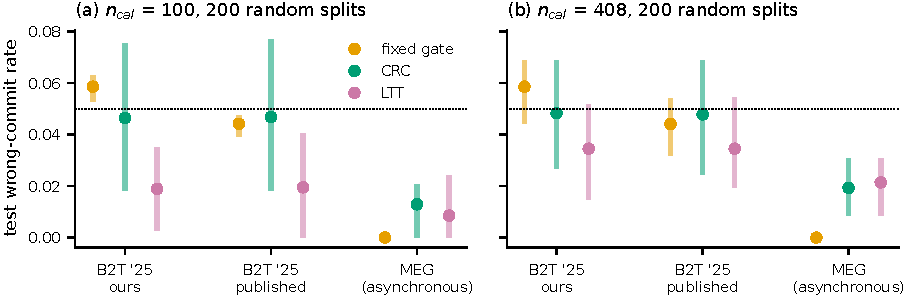
\includegraphics[width=\linewidth]{fig_crc_splits.pdf}
  \caption{\textbf{CRC bounds the mean over splits; LTT bounds the population risk with probability $1 - \delta$} (full-fit pipeline). Test wrong-commit rate over 200 random calibration/test splits of the test pool with (a)~100 and (b)~408 calibration items. Dots: mean; bars: 5th to 90th percentile. Dotted line: $\alpha = 0.05$. A test rate above $\alpha$ in a single split is not a violation of either guarantee.}
  \label{fig:crc}
\end{figure}

\section{Published-gate bonus}
\label{app:bonus}

The gate puts the published sentence on top of our $K$-best list with score = our best score + bonus (\code{published\_margin} in \code{experiments/2026-11-10-b2t25-trust/config.json}). The value 2.0 came with the first commit of that experiment (\code{3fb8154}, 2026-11-10) and never changed; no grid, tuning stage or selection record exists. The data file holds the published sentence but no scores or logits of the published decoder. With the published sentence as the only candidate (score 0, no character confidences), the layer has no signal to rank trials: the fitted policy never commits (threshold 1.01) and every rule equals always offering (18.11 \ewpm{}). Bonus 0 makes the published sentence tie with our top candidate; the layer then commits less and is 1.3 \ewpm{} slower.

\begin{table}[H]
  \centering
  \caption{\textbf{Sensitivity to the published-gate bonus} (guard on). Full fit: plug-in wrong-commit [day-cluster CI], commit, \ewpm{}. Splits A, B: LTT max wrong-commit (commit). Re-splits (50): LTT max mean wrong-commit, share above $\alpha$ (commit).}
  \label{tab:bonus}
  \small
  \begin{adjustbox}{max width=\linewidth}\begin{tabular}{@{}lllllll@{}}
    \toprule
    \textbf{Bonus} & \textbf{Full fit: wrong-commit} & \textbf{Commit} & \textbf{\ewpm{}} & \textbf{Split A} & \textbf{Split B} & \textbf{Re-splits} \\
    \midrule
    \inputrows{generated/tab_bonus.tex}
    \bottomrule
  \end{tabular}\end{adjustbox}
\end{table}

\section{Calibration and the commit trade-off}
\label{app:ece}

\begin{table}[H]
  \centering
  \caption{\textbf{Sentence calibration and error detection} (full-fit pipelines, fixed test sets; 95\% percentile bootstrap at the primary unit). ECE: 15 equal-width bins; the binned ECE is biased upwards, so a percentile interval can lie beside its point value. AUROC: positive class = wrong top-1 sentence. $^{a}$MEG: 2 of 637 top-1 sentences are right, so its AUROC is not informative.}
  \label{tab:ece}
  \small
  \begin{adjustbox}{max width=\linewidth}\begin{tabular}{@{}lllllll@{}}
    \toprule
    \textbf{Condition} & $\boldsymbol{n}$ & \textbf{Top-1 acc.} & \textbf{ECE raw} & \textbf{ECE calibrated} & \textbf{AUROC $1-\hat p$} & \textbf{AUROC guard} \\
    \midrule
    \inputrows{generated/tab_ece.tex}
    \bottomrule
  \end{tabular}\end{adjustbox}
\end{table}

\begin{figure}[H]
  \centering
  \begin{subfigure}[t]{0.32\linewidth}
    \centering
    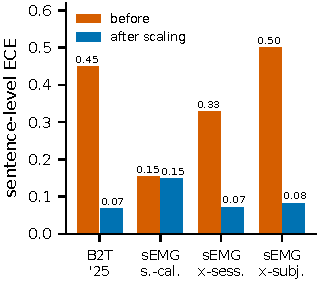
\includegraphics[width=\linewidth]{fig_ece.pdf}
    \caption{Sentence-level ECE.}
    \label{fig:ece}
  \end{subfigure}\hfill
  \begin{subfigure}[t]{0.33\linewidth}
    \centering
    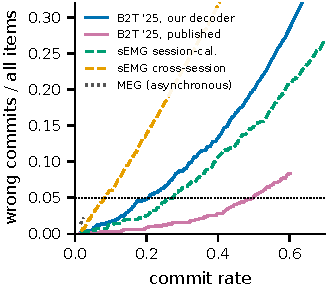
\includegraphics[width=\linewidth]{fig_risk_coverage.pdf}
    \caption{Marginal risk.}
    \label{fig:risk}
  \end{subfigure}\hfill
  \begin{subfigure}[t]{0.33\linewidth}
    \centering
    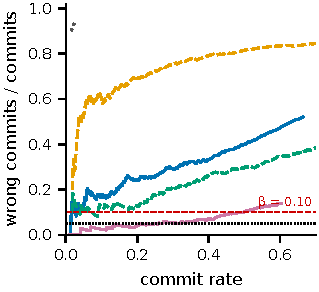
\includegraphics[width=\linewidth]{fig_selective_risk.pdf}
    \caption{Error among commits.}
    \label{fig:selrisk}
  \end{subfigure}
  \caption{\textbf{Calibration and the commit trade-off} (full-fit plug-in pipeline, test sets; not the guaranteed rule). (a)~Sentence ECE before and after temperature scaling. (b)~For each commit threshold: share of test items committed (x) and committed wrongly (y); dotted line: $\alpha = 0.05$. (c)~Error among commits at the same thresholds; dashed line: $\beta = 0.10$. Items blocked by the guard are never committed. Curves start at 10 commits. The error among commits of our decoder falls to 0.1--0.2 only below about 10\% commits; that of the published decoder stays near or below 0.15.}
  \label{fig:calib}
\end{figure}

\section{Ablation}
\label{app:ablation}

\Cref{tab:ablation} refits each variant on the condition's fit data and scores it on the same test items. \emph{No calibration}: no temperature. \emph{Confidence only}: both temperatures fitted, but the beam decodes the raw stream. \emph{No sentence temperature}: the frame temperature is applied before the beam and the sentence calibrator is the identity. \emph{No conformal sets}: \act{offer} shows the fitted top $k$. \emph{LM weight re-tuned}: on sEMG, the LM weight is chosen on fit-A CER with the frame-calibrated streams; on MEG, the validation-tuned beam (3.14 instead of 3.20 \ewpm{}, also no commits). Without the sentence temperature, the wrong-commit rate on our intracortical decoder rose to 0.076 (paired \ci{+0.001}{+0.036}). Without the guard, it fell to 0.036 on our decoder (paired \ci{-0.035}{-0.011}; lower on 9 of 10 days with a difference, sign test $p = 0.021$) and to 0.025 on the published gate (\ci{-0.034}{-0.007}); its AUROC for a wrong top sentence (0.702) was below that of $\hat p_{\mathrm{top1}}$. On sEMG cross-subject, re-tuning the LM weight gave 4.84 \ci{4.28}{5.51} \ewpm{} at top-1 CER 0.360 (instead of 0.479).

\begin{table}[H]
  \centering
  \caption{\textbf{Unified ablation} (full fit; \ewpm{} / wrong-commit rate; point values; ``='': equal to trust).}
  \label{tab:ablation}
  \small
  \begin{adjustbox}{max width=\linewidth}\begin{tabular}{@{}lllllll@{}}
    \toprule
    \textbf{Variant} & \textbf{B2T '25 ours} & \textbf{B2T '25 published} & \textbf{sEMG s.-cal.} & \textbf{sEMG x-sess.} & \textbf{sEMG x-subj.} & \textbf{MEG} \\
    \midrule
    trust (as reported) & 11.55 / 0.059 & 18.77 / 0.044 & 8.02 / 0.004 & 4.68 / 0.004 & 4.08 / 0 & 3.20 / 0 \\
    no calibration & 11.57 / 0.071 & 18.73 / 0.043 & 8.15 / 0.045 & 4.75 / 0.013 & 4.76 / 0.005 & 3.04 / 0.005 \\
    confidence only (raw decoding) & 11.54 / 0.074 & 18.74 / 0.047 & 8.07 / 0.018 & 4.76 / 0.007 & 4.75 / 0 & 3.04 / 0 \\
    no sentence temperature & 11.50 / 0.076 & 18.66 / 0.032 & 8.11 / 0.040 & 4.67 / 0.018 & 4.07 / 0.044 & 3.20 / 0 \\
    no guard & 11.51 / 0.036 & 18.62 / 0.025 & = & = & = & = \\
    no conformal sets & 11.53 / 0.059 & = & 8.07 / 0.020 & = & = & = \\
    \act{offer\_words} off (small grid) & 11.25 / 0.032 & 18.62 / 0.025 & 7.98 / 0.004 & 4.64 / 0 & 4.08 / 0 & 3.20 / 0 \\
    \act{offer\_words} on (small grid) & 11.32 / 0.054 & 18.59 / 0.026 & 7.99 / 0.015 & 4.64 / 0.005 & 4.08 / 0 & 3.20 / 0 \\
    LM weight re-tuned & --- & --- & 8.02 / 0.004 & 4.73 / 0.013 & 4.84 / 0.002 & 3.14 / 0 \\
    gaze typing only & 4.08 & 4.08 & 4.27 & 4.27 & 4.27 & 3.15 \\
    \bottomrule
  \end{tabular}\end{adjustbox}
\end{table}

\section{Data reuse and the fixed-split drift tests}
\label{app:reuse}

\Cref{tab:reuse} gives all 12 reuse comparisons (reused minus clean calibration, test wrong-commit, paired by re-split). The Wilcoxon test over re-splits is valid only conditional on this pool of trials, because the re-splits overlap. The delete-a-day (or delete-a-participant) jackknife recomputes both thresholds without each cluster over all re-splits, so its standard error includes the overlap; it does not refit the pipeline. Holm corrects over the 12 comparisons. Only our decoder shows an effect after Holm (pure CRC and CRC max). With 200 re-splits, our decoder's pure-CRC effect is $+0.0032$ (jackknife Holm-adjusted $p = 0.17$). A single deployment detects a shift of 0.035 (our decoder), 0.038 (published) or 0.040--0.057 (sEMG) with 80\% power.

\begin{table}[H]
  \centering
  \caption{\textbf{Calibration on reused data: all 12 comparisons} (50 re-splits). Diff: mean of reused minus clean test wrong-commit. Wilcoxon over re-splits (conditional on the pool; Holm-adjusted in brackets); sign: re-splits with reused higher / lower; jackknife 95\% CI and $p$ (Holm).}
  \label{tab:reuse}
  \scriptsize
  \begin{adjustbox}{max width=\linewidth}\begin{tabular}{@{}lllllll@{}}
    \toprule
    \textbf{Condition} & \textbf{Rule} & \textbf{Diff} & \textbf{Wilcoxon $p$ (Holm)} & \textbf{Sign} & \textbf{Jackknife CI} & \textbf{Jackknife $p$ (Holm)} \\
    \midrule
    \inputrows{generated/tab_reuse.tex}
    \bottomrule
  \end{tabular}\end{adjustbox}
\end{table}

\paragraph{Fixed-split drift tests.} On the fixed splits (\cref{tab:drift}), clean CRC gave 0.0245 and 0.0600 on our decoder, against 0.0625 when the full-fit pipeline was calibrated on its own fit data. The two clean values above $\alpha$ were within the range of exchangeable splits ($p = 0.21$ and $0.30$). In split A the test rate was above the exchangeable reference ($p = 0.012$; day-stratified $p = 0.014$) but below $\alpha$, where CRC was not binding; after Holm correction over the six tests, none was significant (split A: 0.072). These tests have low power: the 5th--95th percentile range of the reference is 0.029--0.071 on split B and the published gate, and 0.014--0.022 on split A. We claim neither within-day drift nor that reuse caused the old value of 0.0625.

\begin{table}[H]
  \centering
  \caption{\textbf{Fixed splits: clean vs reused calibration} (pure CRC; test sets). Bound: CRC calibration bound $(n\hat R_n(\hat\lambda)+1)/(n+1)$. Exch.\ ref.: mean (5th--95th percentile) over 1,000 random splits of the pooled calibration and test items; $p = (k+1)/(B+1)$, one-sided; Holm over the six tests.}
  \label{tab:drift}
  \small
  \begin{adjustbox}{max width=\linewidth}\begin{tabular}{@{}llllllll@{}}
    \toprule
    \textbf{Data ($n_{\mathrm{test}}$)} & \textbf{Reused} & \textbf{Clean CRC [CI]} & \textbf{Bound} & \textbf{Exch.\ ref.} & $\boldsymbol{p}$ & \textbf{Holm} & \textbf{LTT, pure} \\
    \midrule
    B2T '25 ours, split A (816) & 0.0625 & 0.0245 \ci{0.015}{0.035} & 0.0075 & 0.018 (0.014--0.022) & 0.012 & 0.072 & 0.0270 \\
    B2T '25 ours, split B (816) & 0.0625 & 0.0600 \ci{0.049}{0.071} & 0.0498 & 0.049 (0.029--0.071) & 0.21 & 1.0 & 0.0515 \\
    B2T '25 published, split A (816) & 0.0490 & 0.0478 \ci{0.029}{0.071} & 0.0498 & 0.049 (0.029--0.074) & 0.54 & 1.0 & 0.0294 \\
    B2T '25 published, split B (816) & 0.0490 & 0.0490 \ci{0.030}{0.073} & 0.0498 & 0.050 (0.031--0.074) & 0.50 & 1.0 & 0.0306 \\
    sEMG cross-session (551) & 0.0635 & 0.0563 \ci{0.039}{0.074} & 0.0486 & 0.045 (0.018--0.080) & 0.30 & 1.0 & 0.0309 \\
    sEMG session-cal.\ (551) & 0.0417 & 0.0399 \ci{0.025}{0.056} & 0.0486 & 0.047 (0.018--0.082) & 0.60 & 1.0 & 0.0218 \\
    \bottomrule
  \end{tabular}\end{adjustbox}
\end{table}

\section{Online re-calibration}
\label{app:online}

An online controller re-tunes the commit threshold from user feedback, with a long-run guarantee for any sequence of items (\cref{tab:online}). On the fixed splits (warm start on the clean calibration data, then the test data in file order), the online controllers kept the long-run rate at 0.0245--0.0527 (Brain-to-Text '25) and 0.0381--0.0526 (sEMG), at \ewpm{} within 0.06 of offline CRC (\cref{tab:online-results}). The bounds say nothing about short windows: the largest rate in a rolling window of 50 items was 0.06--0.18. When only noticed errors were fed back (delay 10), \texttt{aci} reached 0.027--0.058 while its certificate on the observed losses was at most 0.0509: silent errors look correct to the controller. The sEMG online order is participant by participant, not a time sequence.

\begin{table}[H]
  \centering
  \caption{\textbf{Online re-calibration methods.} $L_t$: realised loss of item $t$; $T$: items in the sequence; $d$: feedback delay. The \texttt{aci} variants bound the long-run average of the \emph{observed} losses for any sequence; \texttt{window} and \texttt{decay} have no guarantee under shift.}
  \label{tab:online}
  \small
  \begin{adjustbox}{max width=\linewidth}\begin{tabular}{@{}llll@{}}
    \toprule
    \textbf{Method} & \textbf{Update} & \textbf{Guarantee} & \textbf{Feedback} \\
    \midrule
    \texttt{window} & CRC on the last $N = 200$ items with known truth & none under shift & full \\
    \texttt{decay} & weighted CRC on all past items, weights $0.99^{\text{age}}$ & none under shift & full \\
    \texttt{aci} & $\lambda_{t+1} = \max(0, \lambda_t + \eta(L_t - \alpha))$, $\eta = 0.05$ \citep{gibbs2021aci,angelopoulos2023pid,feldman2023rolling} & $\frac1T\sum_t L_t \le \alpha + \frac{\lambda_{T+1} - \lambda_1}{\eta T}$; a priori $\alpha + \frac{1 - \lambda_1 + \eta(1+d)}{\eta T}$ & realised only \\
    \texttt{aci\_window} & window CRC at level $\alpha_t$; $\alpha_{t+1} = \min(2\alpha, \alpha_t + \gamma(\alpha - L_t))$, $\gamma = 0.005$ & $\frac1T\sum_t L_t \le \alpha + \frac{\alpha_1 - \alpha_{T+1}}{\gamma T}$ & full + realised \\
    \bottomrule
  \end{tabular}\end{adjustbox}
\end{table}

\begin{table}[H]
  \centering
  \caption{\textbf{Online re-calibration on the fixed splits} (long-run test wrong-commit rate). Cert.\ / a priori: \texttt{aci} bound after the fact and in advance.}
  \label{tab:online-results}
  \small
  \begin{tabular}{@{}llllll@{}}
    \toprule
    \textbf{Data} & \texttt{window} & \texttt{decay} & \texttt{aci} & \texttt{aci\_window} & \textbf{Cert.\ / a priori} \\
    \midrule
    B2T '25 ours, split A & 0.0245 & 0.0257 & 0.0270 & 0.0245 & 0.043 / 0.068 \\
    B2T '25 ours, split B & 0.0478 & 0.0453 & 0.0527 & 0.0490 & 0.053 / 0.066 \\
    B2T '25 published, split A & 0.0429 & 0.0392 & 0.0478 & 0.0453 & 0.048 / 0.059 \\
    B2T '25 published, split B & 0.0441 & 0.0392 & 0.0478 & 0.0453 & 0.048 / 0.059 \\
    sEMG cross-session & 0.0472 & 0.0381 & 0.0526 & 0.0490 & 0.053 / 0.081 \\
    sEMG session-cal. & 0.0490 & 0.0454 & 0.0490 & 0.0490 & 0.049 / 0.072 \\
    \bottomrule
  \end{tabular}
\end{table}

\section{LM leakage check}
\label{app:leakage}

A near variant is a sentence within a character edit distance of 0.25 times its length, after normalisation, in the 600,000-sentence training slice of the English character LM. Of the 1,717 unique Brain-to-Text '25 cue sentences, 22 have an exact copy and 310 an exact or near variant; of the 551 sEMG test sentences, none has an exact copy and 295 have a near variant (Tatoeba is heavily templated). Rebuilding the LMs without these sentences changed 2 of 1,628 top-1 sentences on Brain-to-Text '25 and sEMG trust \ewpm{} by at most $-0.04$, and no wrong-commit rate by more than 0.002. Rebuilding does not remove the advantage of templated test sentences, which are easier to decode, so we also scored the 256 sEMG test sentences without a near variant: trust \ewpm{} fell from 8.02, 4.68 and 4.08 to 6.97, 4.08 and 3.69; trust minus gaze typing became \ci{+1.82}{+3.92}, \ci{-0.37}{+0.27} and \ci{-0.66}{-0.23}; always-commit wrong-commit rates rose to 0.664, 0.961 and 0.992; and the layer stayed safe (1 wrong commit in 256 sentences; one-sided upper bound 0.018). On Brain-to-Text '25, excluding the 147 test trials with a near variant gave a trust wrong-commit rate of 0.055 (all: 0.059) on our decoder and 0.042 (0.044) on the published gate.

\section{MEG decoder and sentence-level limits}
\label{app:meg}

We split 19 participants' data by a hash of the sentence text into 101 training, 11 validation and 17 test sentences (637 test instances); the same people appear in all splits, and no test sentence is in training or LM text. All trust parameters are fitted on the 437 validation instances (6 sentences fit, 5 calibrate in the deployment protocol). The decoder is a convolutional front end (320 channels) followed by 4 Conformer layers of width 256 \citep{gulati2020conformer}, trained with CTC and a keystroke auxiliary loss that uses key times as training labels. At inference it takes the MEG segment (first key $-$ 0.4\,s to last key press $+$ 0.5\,s), its length and the participant index; it has no key input (the published asynchronous decoder takes the same inputs but uses no key-time labels \citep{zhang2026brain2qwertyv2}). The trust harness keeps the beam settings of the earlier harness; with the validation-tuned beam the layer also committed nothing.

\paragraph{Sentence-grouped calibration.} Instances of one sentence are dependent, so a guarantee for new sentences needs the sentence as the unit: sentence-level CRC needs at least 19 calibration sentences and LTT 45, while the data set has 5 clean calibration, 11 validation and 17 test sentences. Sentence-level CRC was therefore infeasible and never committed. With calibration and test sentences disjoint, instance-level CRC gave mean test rates of 0.016--0.019 (never above $\alpha$ in 1,000 splits each with 5, 8 or 11 calibration sentences), but only 2.4\% of instances were eligible and 0.91--0.94 of the commits were wrong; the max rule committed nothing. Two-way MEG intervals: trust minus gaze typing \ci{-0.10}{+0.25} (sentences \ci{-0.04}{+0.15}, participants \ci{-0.08}{+0.22}); gaze typing with word completion was faster \ci{-1.13}{-0.64}. A synchronous control decoder with oracle key times gave the same trust result; over trials (instead of sentences) its difference to gaze typing excluded 0, which shows how trial-level intervals overstate MEG gains.

\section{Stream format, standards and audit log}
\label{app:format}

\paragraph{Fields and rules.} Besides the log-probability array, frame times, vocabulary, vocabulary type (\code{char}, \code{key}, \code{phoneme}, \ldots) and blank index, optional fields give the frame period, latency, producer and a \code{meta} object with named key prefixes (\code{device.*}, \code{decoder.*}, \code{lm.*}, \code{calibration.*}, \code{adapter.*}). A field is interpreted as a probability only if the stream declares it as one in \code{calibration.*}. Raw signals and direct identifiers stay out of the stream. NWB \citep{rubel2022nwb}, BCI2000 and OpenViBE \citep{schalk2004bci2000,renard2010openvibe}, IEEE P2731 and P2794 \citep{ieeep2731,ieeep2794,eiber2021reporting} and decoder benchmarks \citep{jayaram2018moabb,banville2026neuralbench} each cover part of the stack; none defines a per-frame decoded-output format with confidence semantics.

\paragraph{Serialisations, conformance and adapters.} The reference serialisations are an NPZ file and a JSON Lines streaming form. A conformance suite runs 60 checks, each tied to a specification clause, at three cumulative levels (\emph{core}, \emph{trust-ready}, \emph{provenance}); it ships 52 golden test vectors, and the reference consumer passes all 52. The adapters have 412 (intracortical), 568 (sEMG) and 156 (MEG) physical lines of Python. Mapping the decoders into the stream needed no change to the frame core of v0.1, a Development release written by the same authors.

\begin{table}[H]
  \centering
  \caption{\textbf{Devices, data and streams.} All data sets are public.}
  \label{tab:devices}
  \small
  \begin{adjustbox}{max width=\linewidth}\begin{tabular}{@{}llll@{}}
    \toprule
    & \textbf{Intracortical (speech)} & \textbf{Forearm sEMG (keys)} & \textbf{MEG (typing)} \\
    \midrule
    Data set (licence) & B2T '25 copy task (CC0) & Toronto sEMG (CC BY 4.0) & SpanishBCBL (CC BY-NC 4.0) \\
    Participants & 1 (T15, ALS) & 19 (healthy typists) & 19 (healthy typists) \\
    Test unit & 816 trials, 14 days & 551 composed sentences & 637 instances of 17 sentences \\
    Decoder & published online RNN; own phoneme-to-word decoder & own CNN & own asynchronous ConvCTC \\
    Stream vocabulary & \code{phoneme} (CTC, 41 tokens) & \code{key} (W3C codes) & \code{char} (CTC) \\
    Frame & 80\,ms & one per key press & 40\,ms \\
    Commit decision tested? & yes & weakly (0--9\% committed) & no (no right top-1) \\
    \bottomrule
  \end{tabular}\end{adjustbox}
\end{table}

\begin{figure}[H]
  \centering
  \begin{adjustbox}{max width=0.85\linewidth}\input{\figdir tikz-architecture.tex}\end{adjustbox}
  \caption{\textbf{Architecture.} Each device's decoder emits a stream through a small adapter. The trust layer reads the stream: it calibrates confidence, builds candidate sentences, and chooses an action under a risk-control rule. The user's corrections and picks (dashed) can feed online re-calibration. Decisions can be written to a hash-chained audit log that stores no raw signals.}
  \label{fig:arch}
\end{figure}

\paragraph{Audit log.} Each decision can be appended to a JSON Lines log. Context entries are content-addressed and hold the adapter, decoder, LM, calibration and policy versions; decision entries hold the action, scores, a hash of the stream and its frame range; correction entries link to the decision they correct. Each entry stores the hash of the previous entry, so any edit, deletion or reordering breaks the chain; a separately stored head anchor detects truncation. The log stores no raw signals and is tamper-evident, not tamper-proof (no signature in v0). A replay of the 816 Brain-to-Text '25 test trials (1,723 entries) passed verification, recorded the same wrong commits as the harness, and detected every tampering case we tried, at about 0.1\,ms and 1.1\,kB per decision (\cref{fig:audit}).

\begin{figure}[H]
  \centering
  \fbox{\begin{minipage}{0.94\linewidth}\footnotesize\raggedright
  \textbf{Wrong commit} \texttt{dec-000041-ed60b4bd} (entry 44, hash \texttt{8cf2c6c67053b185...})\\
  Committed: ``who you never expect to when''\\
  Correction (known cue sentence, hash-linked): ``who you never expect to win''; 2 character edits, 1 word edit\\
  Scores: $\hat p_{\mathrm{top1}}$ 0.5814, set size 3, guard risk 0.2857; reason: $\hat p_{\mathrm{top1}} \ge 0.50$\\
  Input: stream \texttt{1b4b60e8e4950710...}, frames [0, 335], item \texttt{b2t25-test-trial-196}\\
  Decoder: published online RNN + our phoneme-to-word decoder; LM: Tatoeba character 6-gram + word unigram + CMUdict\\
  Calibration \texttt{cal-692fb52a73417552}: $\tau_f$ 3.7809, $\tau_s$ 4.5551; policy \texttt{pol-2eaa4ff51919527a}: commit threshold 0.5
  \end{minipage}}
  \caption{\textbf{One entry of the audit report} (B2T '25 replay, full-fit plug-in layer, our decoder; public CC0 copy-task cue, not the participant's own words). Hashes are shortened.}
  \label{fig:audit}
\end{figure}

\section{What each calibration set was and was not used for}
\label{app:separate}

Both guarantees need the parts that define $s_i$ (temperatures, conformal sets, guard and policy thresholds) to be fitted on data disjoint from the calibration items. Four exceptions remain. (1) Brain-to-Text '25, fixed splits: the word-decoder grid (LM weight, edit penalty, word bonus; 12 points) was tuned on a random 400 of the 812 fit trials, so 187 and 189 of the 401 calibration trials of splits A and B were in that tuning set; re-tuning on fit-A only selected the same setting in both splits. (2) Brain-to-Text '25, random re-splits and time-ordered tests: the same 400 trials are permuted into fit-A, calibration and test parts (about 100 into calibration and 200 into test per re-split); the re-tune check covers only the two fixed splits, so this overlap is not checked. The grid is small, so the bias is likely small. (3) MEG: the decoder checkpoint was selected by validation CER, and the validation sentences include the 5 calibration sentences. (4) sEMG session-calibrated: calibration and test logits come from two cross-fitted decoder runs, so their score functions differ by design. LTT also needs i.i.d.\ sampling; our random splits sample without replacement from a finite pool, which makes its binomial test conservative.

\section{Controls}
\label{app:controls}

\Cref{tab:controls} gives the commits on the Brain-to-Text '25 control streams for the frozen configurations tagged \code{paper1-v3-frozen-config} (frozen v3) and \code{paper1-v4-frozen-config} (frozen v4). With the guard, the split-A pipeline committed no frame-shuffled or uniform stream on either decoder, and its real-trial test rate was unchanged (0.0245 ours, 0.0294 published; a refit that reproduces the committed values). On Brain-to-Text '25, the guard risk separated frame-shuffled and uniform streams from real ones with AUROC 0.981 and 0.998. On MEG the layer committed nothing on real input either, so its zero commits on controls carry no information; the guard risk separated shuffled MEG, zero input and uniform streams (AUROC 0.92, 1.00, 1.00), but not frame-shuffled streams (0.47) (\cref{fig:null}c).

\begin{table}[H]
  \centering
  \caption{\textbf{Commits on the Brain-to-Text '25 control streams} (300 test trials; split-A pipeline unless marked). Other trial: the real stream of a different sentence (intent mismatch). Frame-shuffled and uniform streams carry no neural information, so every commit on them is wrong. Uniform WC: wrong-commit rate on uniform streams.}
  \label{tab:controls}
  \small
  \begin{adjustbox}{max width=\linewidth}\begin{tabular}{@{}lllllll@{}}
    \toprule
    \textbf{Decoder} & \textbf{Configuration} & \textbf{Real} & \textbf{Other trial} & \textbf{Frame-shuffled} & \textbf{Uniform} & \textbf{Uniform WC} \\
    \midrule
    \inputrows{generated/tab_controls.tex}
    \bottomrule
  \end{tabular}\end{adjustbox}
\end{table}

\begin{figure}[H]
  \centering
  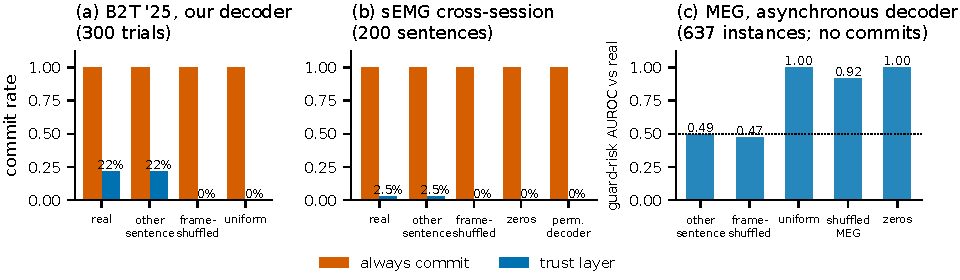
\includegraphics[width=\linewidth]{fig_null_audit.pdf}
  \caption{\textbf{Controls} (full-fit plug-in layer with the guard). (a, b)~Commit rate of always commit (orange) and the trust layer (blue) on real input, the intent-mismatch control (other sentence) and signal-destroying controls: (a)~B2T '25, our decoder, 300 test trials; (b)~sEMG cross-session, 200 test sentences. (c)~MEG, 637 instances: AUROC of the guard risk for separating each control from real input (dotted line: chance).}
  \label{fig:null}
\end{figure}

\section{How to state the guarantees}
\label{app:guarantees}

With LTT and the max rule (primary): ``if the calibration sentences and later sentences are i.i.d.\ draws from the same mix of sessions, and the calibration sentences fitted no other part of the system, then, with probability at least 0.9 over the choice of the calibration sentences, the long-run share of sentences committed wrongly, averaged over that mix of sessions, is at most 0.05''. It is not a statement about each session; in our data one day ran at about 0.10. With CRC: ``under exchangeability and the same separation, averaged over the choice of the $n$ calibration sentences and over a new sentence, the probability that the new sentence is committed wrongly is at most 0.05''; a single calibration set can exceed 0.05. With joint LTT: ``with probability at least 0.9, both the long-run wrong-commit share is at most $\alpha$ and the long-run share of wrong sentences among committed sentences is at most $\beta$'' (i.i.d.\ calibration sentences, separate from all fitted parts). With SGR: the bound of Geifman and El-Yaniv (2017, Theorem 3.2) on the error among accepted items, with probability at least 0.9, for i.i.d.\ calibration sentences separate from all fitted parts; its thresholds are chosen by bisection on the same data. With adaptive online re-calibration: ``for any sequence of sentences, the average observed wrong-commit rate over the first $T$ sentences is at most $0.05 + (1 - \lambda_1 + \eta(1+d))/(\eta T)$''. On MEG the unit is the sentence, and none of these statements applies to new sentences. All statements count only the errors that the system observes, so each should be reported with the measured silent-error rate.

\section{Data sets and licences}
\label{app:licences}

\begin{table}[H]
  \centering
  \caption{\textbf{Data sets, resources and licences.}}
  \label{tab:licences}
  \small
  \begin{tabular}{@{}p{4.3cm}p{2.4cm}p{3.6cm}p{4.2cm}@{}}
    \toprule
    \textbf{Data set / resource} & \textbf{Licence} & \textbf{Use} & \textbf{Note} \\
    \midrule
    SpanishBCBL \citep{levy2026brain2qwerty,spanishbcbl} & CC BY-NC 4.0 & MEG decoder training and evaluation & Research only; weights trained on it are not released for commercial use \\
    Brain-to-Text '25 copy-task logits \citep{card2024accurate,card2025data} & CC0 1.0 & intracortical trust evaluation & Companion code has no licence; we wrote our own loader \\
    Toronto sEMG typing \citep{achituve2025emg,achituve2024data} & CC BY 4.0 & sEMG decoder and trust evaluation & Baseline code (CC BY-SA 4.0) not used \\
    Tatoeba English / Spanish sentences & CC BY 2.0 FR (some CC0) & character LMs; composed sEMG sentences & Sentences from Tatoeba (\url{https://tatoeba.org}), by the Tatoeba contributors \\
    CMUdict (commit 7479086) & BSD-2-Clause style & phoneme-to-word lexicon & Copyright notice kept \\
    Brain2Qwerty code (Meta) & CC BY-NC 4.0 & read only, not copied & Our decoders are our own implementations \\
    Fidetype code and specification & Apache-2.0 & all methods & --- \\
    \bottomrule
  \end{tabular}
\end{table}


\end{document}
